
\documentstyle[color,changebar,cprog,epsbox,tabular,shadow,ascmac,graphicx]{jfspec}
\makeindex
\topmargin    -1.5cm
\headheight      1pc
\headsep         2pc
\textheight     60pc
\footskip        3pc
\footheight      1pc
\oddsidemargin   0pc
\evensidemargin  0pc
\textwidth      38pc
\columnsep       2pc
\cprogbaselineskip 1ex
\partopsep       0pc
\parsep          0pc
\itemsep         0pc
\parskip         0pc
\topsep          0pc
\renewcommand{\topfraction}{1}
\renewcommand{\floatpagefraction}{1}
\renewcommand{\dbltopfraction}{1}
\renewcommand{\dblfloatpagefraction}{1}
\renewcommand{\textfraction}{0}
\renewcommand{\bottomfraction}{0}
%\renewcommand{\floatsep}{1pc}        %$B%U%m!<%H4V$N5wN%(B
%\renewcommand{\textfloatsep}{1pc}    %$B%U%m!<%H$HK\J84V$N5wN%(B [t,b]
%\renewcommand{\dblfloatsep}{1pc}     %2$BCJAH$N>l9g$N(B \floatsep
%\renewcommand{\dbltextfloatsep}{1pc} %2$BCJAH$N>l9g$N(B \textfloatsep
%\renewcommand{\intextsep}{1pc}       %$B%U%m!<%H$HA08e$NK\J8$H$N5wN%(B [h]
\renewcommand{\indexspace}{}

\title{\shabox{\LARGE EMAX7/ACAP (IMAX3) Architecture Handbook\newline -- In-Memory Accelerator eXtension --}}
\author{Nara Institute of Science and Technology\\Computing Architecture Laboratory\\Accelerator Group}
\date{\renewcommand{\arraystretch}{0.4}\tabcolsep 0.1pc
\sboxsep=5pt \sdim=2pt \sboxrule=.4pt
\begin{tabular}{lrrr}
\multicolumn{4}{r}{EMAX7SPC-0001}\\
Ver.0.1: & Sep. &  1 & 2023\\
Ver.0.2: & Apr. &  1 & 2024\\
\end{tabular}}

\begin{document}
\maketitle
\tableofcontents
\listoffigures
\listoftables


\chapter{IMAX3 Hardware}

\section{Chiplet and Vector Length}

\begin{figure}[htbp]
\center
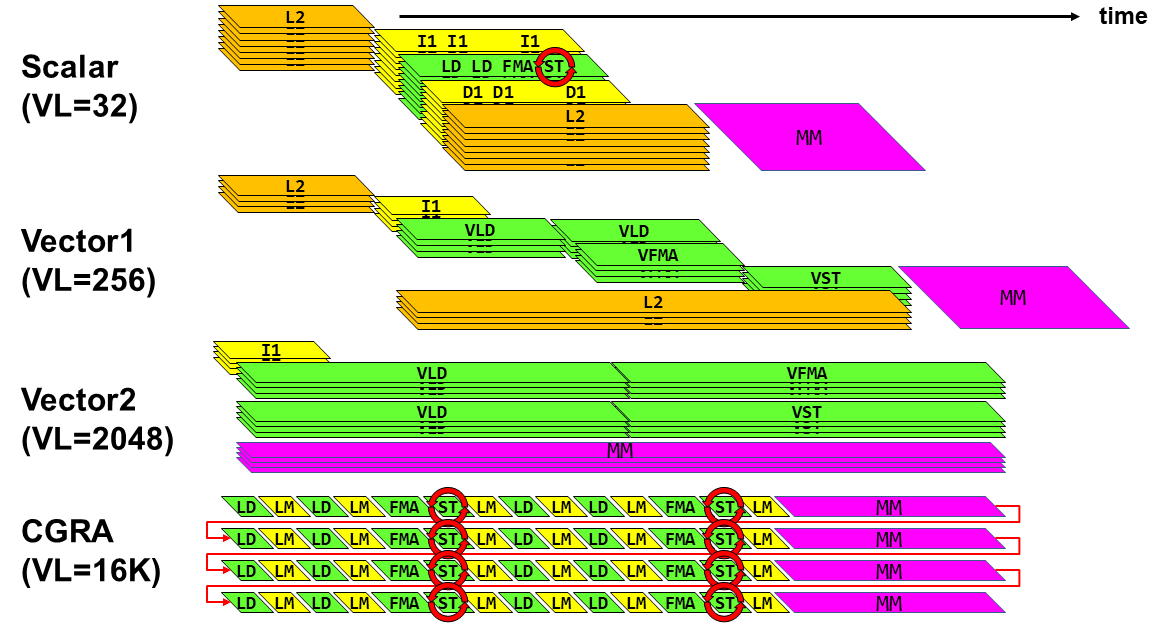
\includegraphics[angle=270,origin=b,width=0.85\textwidth]{fig01.eps}
\caption{\label{fig:vl}Variation of Vector Length}
\end{figure}

\begin{figure}[htbp]
\center
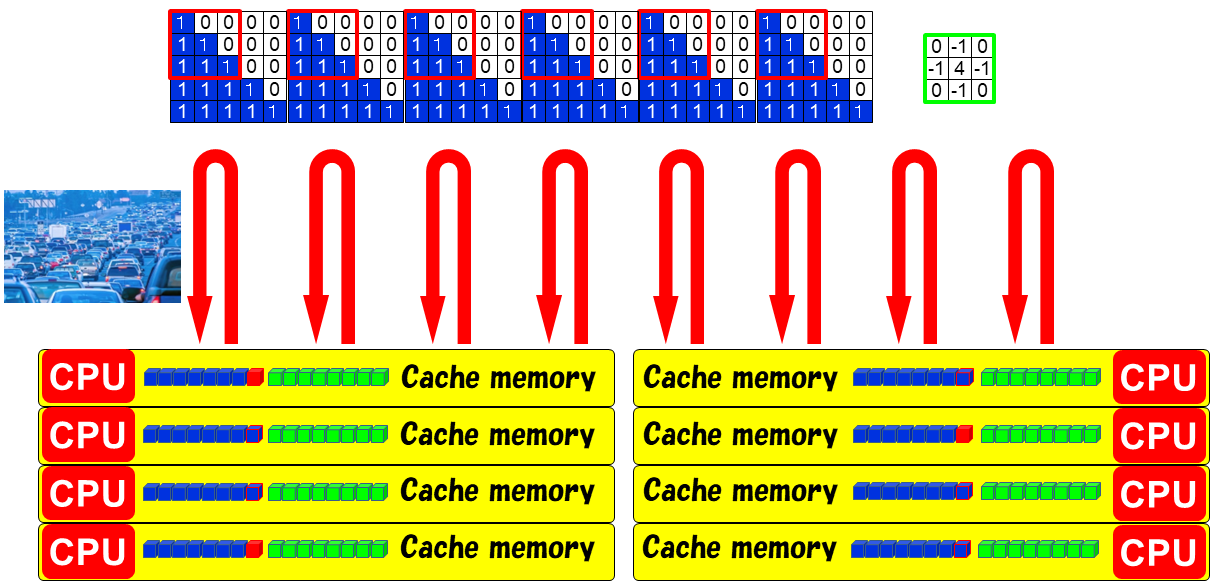
\includegraphics[angle=270,origin=b,width=0.32\textwidth]{fig02.eps}
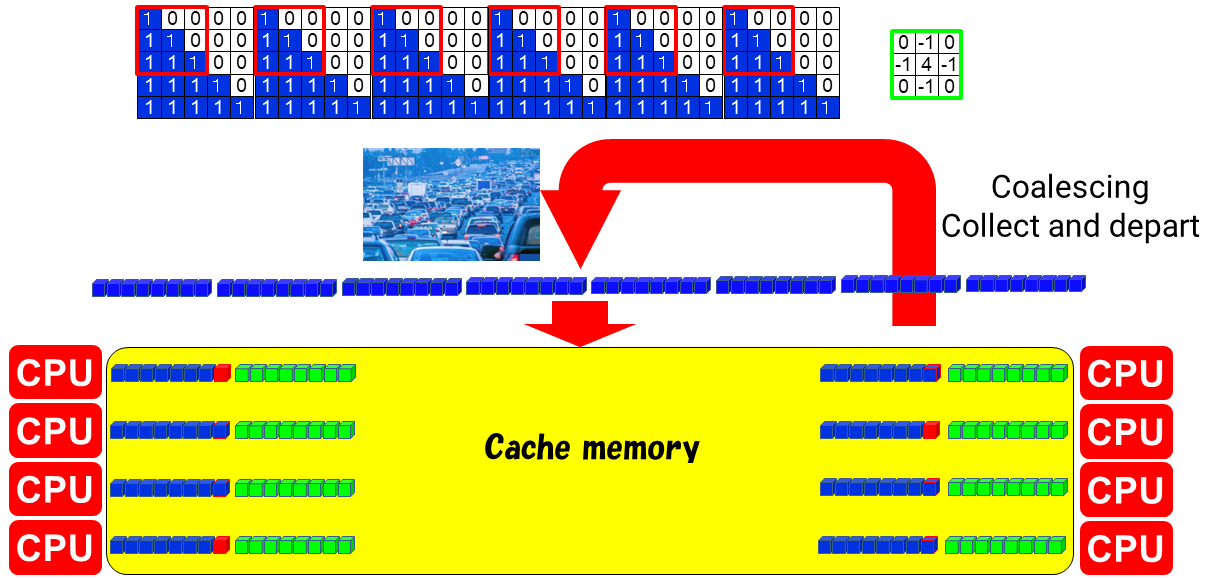
\includegraphics[angle=270,origin=b,width=0.32\textwidth]{fig03.eps}
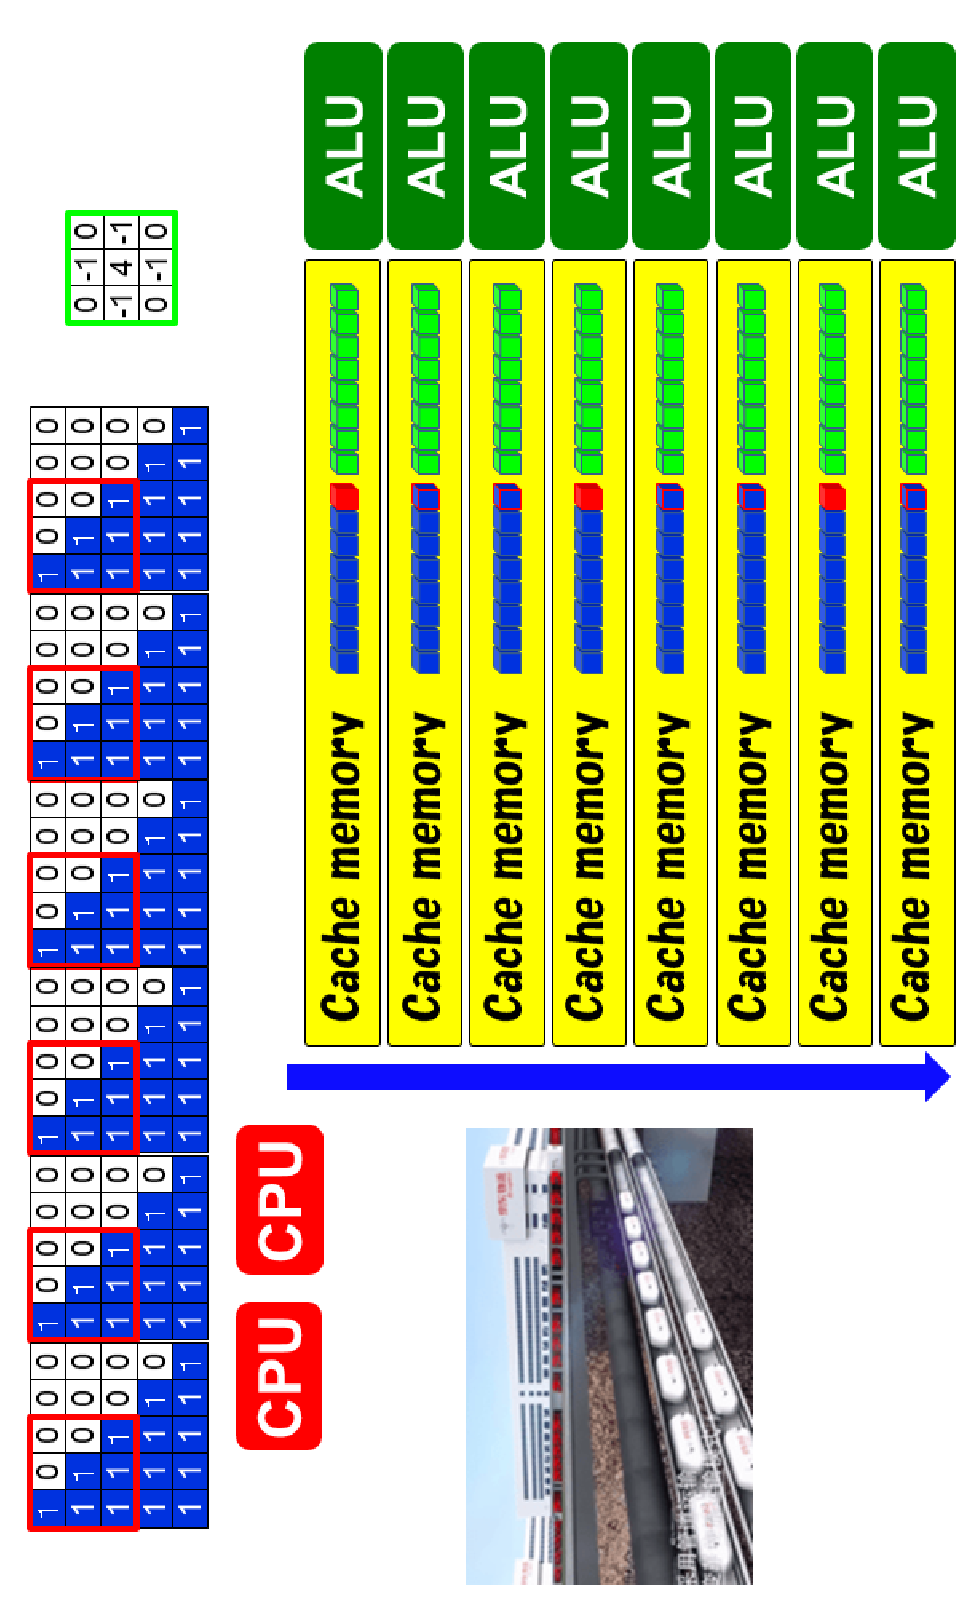
\includegraphics[angle=270,origin=b,width=0.32\textwidth]{fig04.eps}
\caption{\label{fig:comp}Multicore system, GPGPU and CGRA}
\end{figure}

���åץ�åȲ��ˤϡ����å״֥ǡ���ž�������Хإåɤ�Ǿ������뤿��ˡ���ʬ��
�٥��ȥ�Ĺ��ɬ�פǤ��롥�����ơ�IMAX3�ϡ����åץ�åȻظ��������ƥ�����Ǥ�
�롥��\ref{fig:vl}�ϡ��ϡ��ɥ����������ȥ٥��ȥ�Ĺ�δط��Ǥ��롥32�������٤�
SIMD�ϡ�������ץ����å�����ܤǤ��롥256���ǰʾ��SIMD�ϡ��٥��ȥ�ȸƤФ�
�롥���Τ������٥��ȥ�1�ϡ�����å���������³����Ƥ��롥�٥��ȥ�2�ϡ���
��������ľ�뤹�뤳�Ȥǡ��٥��ȥ�Ĺ��2048���٤ޤdz�ĥ�Ǥ��롥�����ơ�CGRA
�ϡ�ALU�ȡ�64KB�Υ���å������Υ���ɥ��å���¤�ˤ��뤳�Ȥǡ��٥��ȥ�Ĺ
��16K���٤ޤdz�ĥ�Ǥ��롥�Ե�§�ʥ��������ѥ�����򥭥�å������˥��ץ�
�벽���뤳�Ȥǡ��ᥤ�����ϵ�§Ū�ʥ��������ѥ�����ˤ���®ư���ݻ���
���롥

��\ref{fig:comp}�ˡ�ŵ��Ū�ʼ¹ԥ�ǥ�򼨤���1��μ֤���1�Ĥ�CPU�Ǥ����
���ꤹ�롥�Ŀ��Υǡ��������ϲ������п��Υǡ������ŤߤȤ��롥���٤Ƥ�CPU�ϡ�
���Ȥ�Ʊ���ǡ����Ǥ��äƤ⡤����å��� �������­���Ƥ���ǡ������������
���Ȥ��롥���������ǡ������������夹�뤫��ͽ¬���뤳�ȤϤǤ��ʤ���GPGPU��¿
���Υ�������ܤ��Ƥ��롥�����ơ���ξ�ϡ���ȯ���˲�ǽ�ʸ¤����󤷤��Ե����롥
��ȯ����������礹�뤳�Ȥǡ����ڤ���¤��뤳�Ȥ��Ǥ��롥 ����������Ū�Ϥ�ʬ
�����Ƥ����硤�н�Ϻ���Ǥ��롥����Ǥ��뤫�ɤ����ϡ��ץ�����ߥ󥰥�����
�˰�¸���롥�����ơ���¦��IMAX�Ǥ��롥�����ˡ������Ĥ���CPU�����롥��¿����
����å������ϡ�����ǡ�����������˹Ԥ����ȤϤʤ���CPU�����󶡤����ǡ�
�����Ԥġ�CPU���п��ν��̥ǡ�������٤������Ǥ����ǡ����̿��̤Ⱦ��񥨥ͥ륮��
��︺�Ǥ��롥

\section{Independent network for memory and execution}

\begin{figure}[htbp]
\center
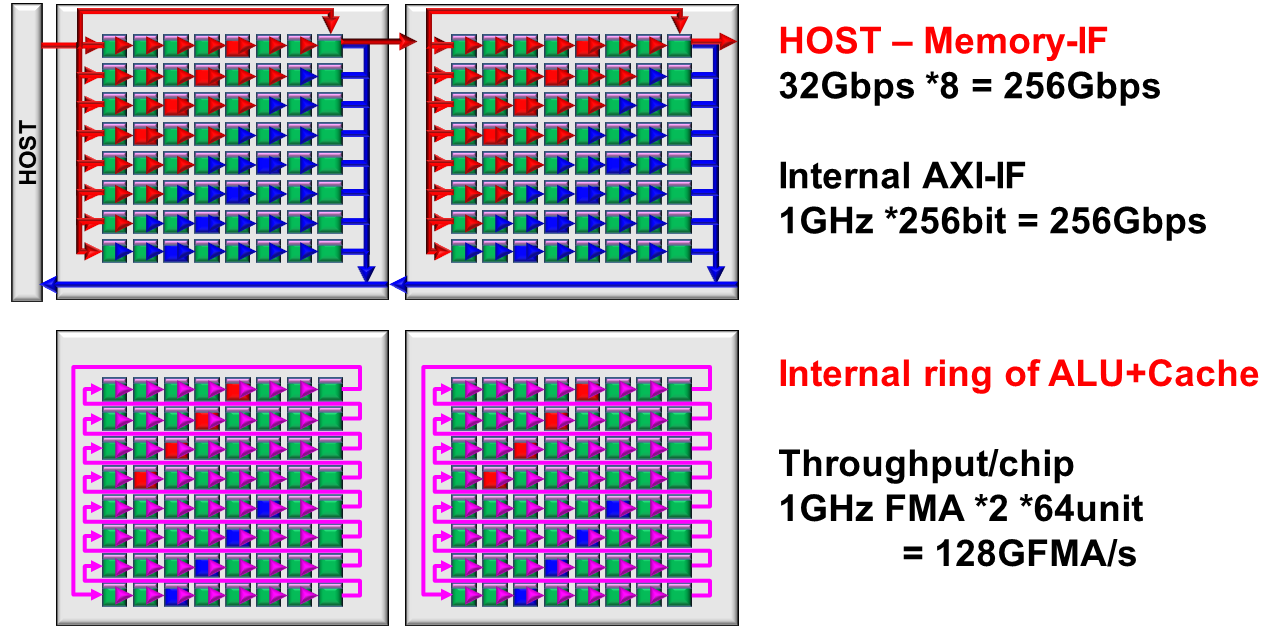
\includegraphics[angle=270,origin=b,width=0.80\textwidth]{fig05.eps}
\caption{\label{fig:mesh}Execution network and Memory network}
\end{figure}

\begin{figure}[htbp]
\center
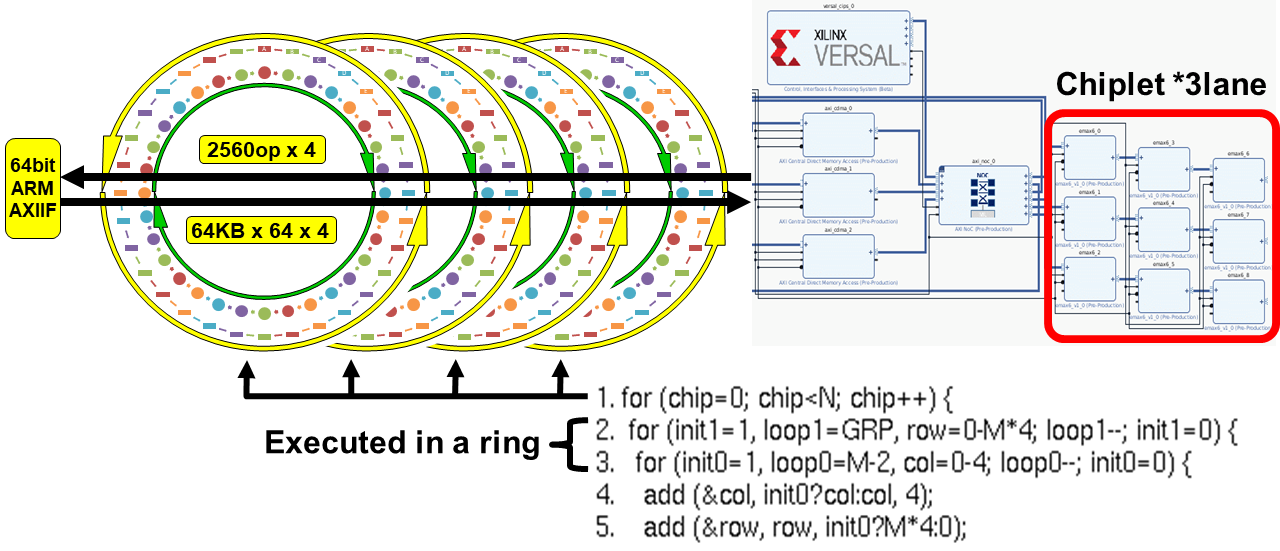
\includegraphics[angle=270,origin=b,width=0.80\textwidth]{fig06.eps}
\caption{\label{fig:ring}IMAX2 multichip structure}
\end{figure}

\begin{figure}[htbp]
\center
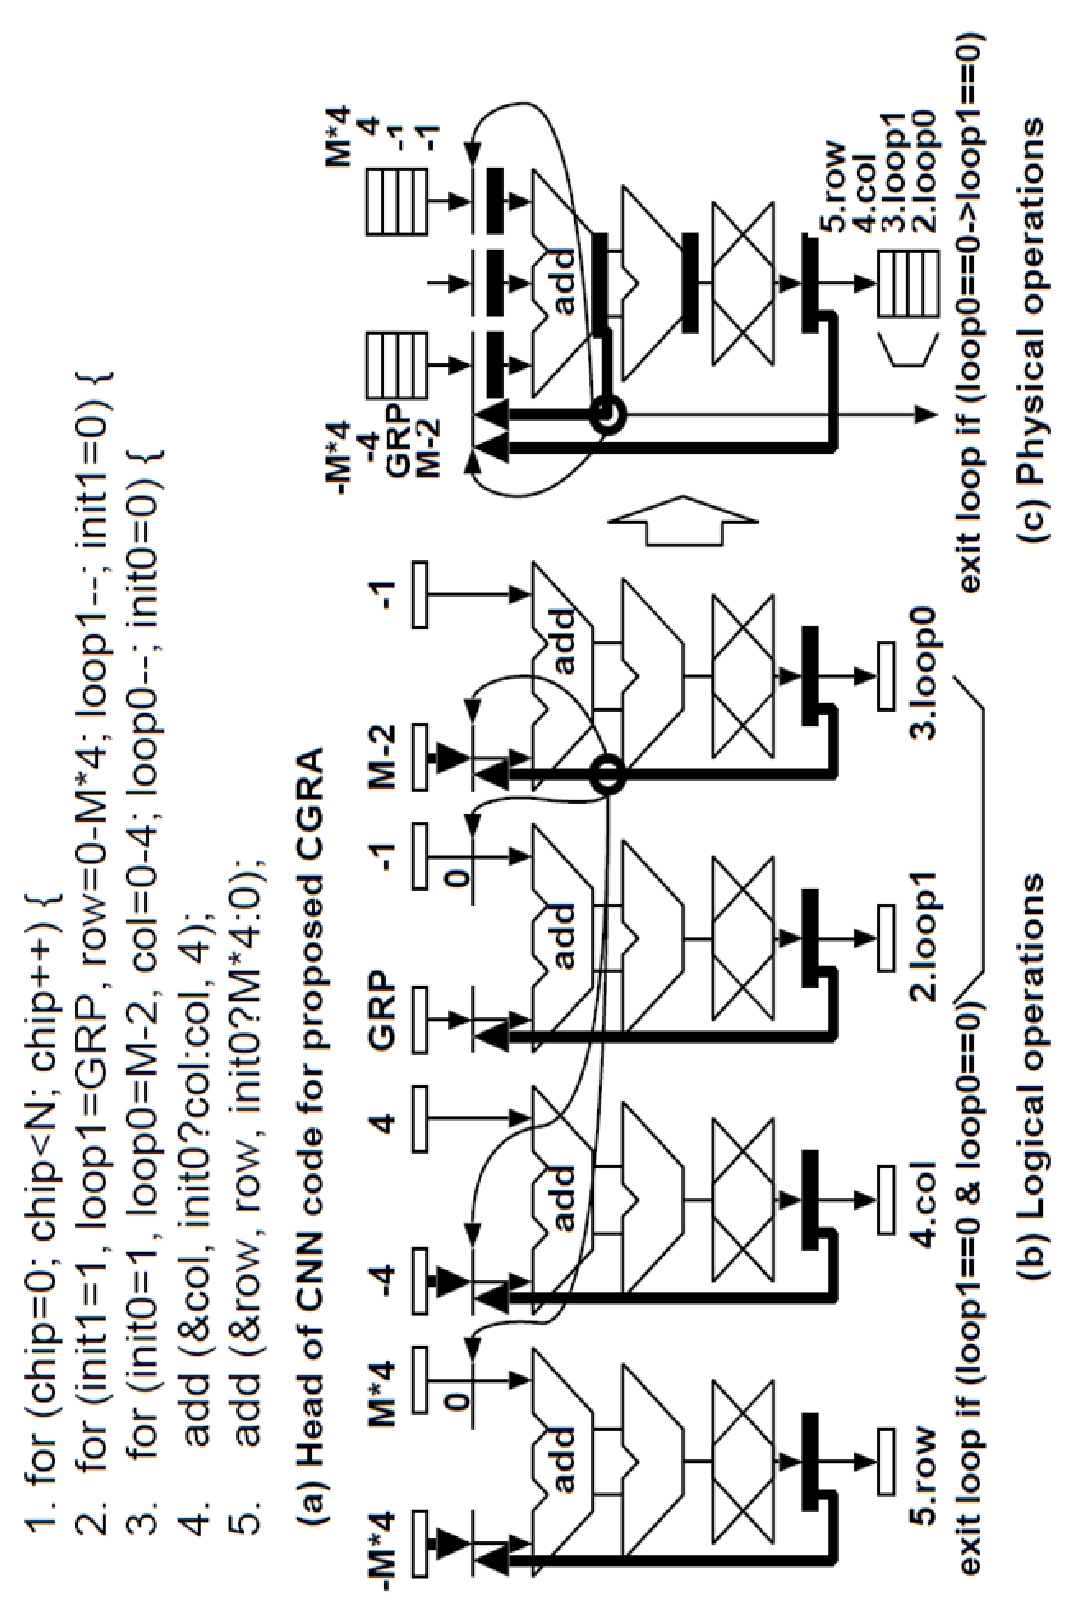
\includegraphics[angle=270,origin=b,width=0.80\textwidth]{fig30.eps}
\caption{\label{fig:loopctrl}Burst execution of triple loops}
\end{figure}

\begin{figure}[htbp]
\center
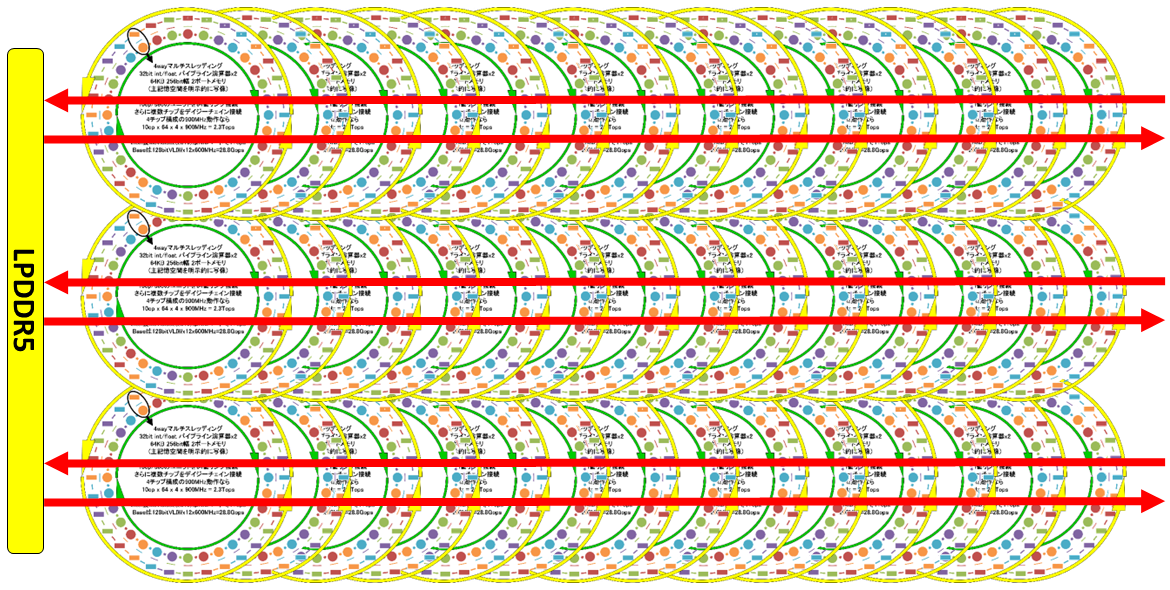
\includegraphics[angle=270,origin=b,width=0.80\textwidth]{fig33.eps}
\caption{\label{fig:multilane}IMAX3 multilane structure}
\end{figure}

��\ref{fig:mesh}�˼����褦�ˡ�IMAX2�ˤ�2����Υͥåȥ�������롥8�ĤΥ�˥�
�Ȥ򥰥롼�ײ��������ꥤ�󥿡��ե�������������³���뤳�Ȥˤ�ꡤ�쥤�ƥ�
��û�̤��Ƥ��롥�黻�ˤϡ��ƥ��å����64�ĤΥ�˥åȤ���󥰾�����³���졤��
�������Τ褦�ˡ��黻�ȥ������������ȹ礻���ѹ��Ǥ��롥��󥰹�¤�ϥ���
�󥷥�׻�����Ω�ġ��ޥåԥ󥰤��줿���򥹥饤�ɤ����뤳�Ȥǡ�ALU�ȥ����
�������Υڥ����ѹ��Ǥ�������å��������Υǡ�����¿���������ѤǤ��롥
�ޤ�����\ref{fig:ring}�˼����褦�ˡ���ư�����С��إåɤ�︺���뤿��ˡ��ȥ�
�ץ�롼�פ�IMAX2�˰��٤˥ޥåԥ󥰤Ǥ��롥�dz��롼�פ�ʣ�����åפ˥ޥåԥ�
�����졤��¦�Σ��ť롼�פϳƥ��åפ˥ޥåԥ󥰤���롥��\ref{fig:loopctrl}�ϡ�
�ȥ�ץ�롼�������4�Ĥ�������˥å�(1�Ĥ�ʪ����˥å�)���¹Ԥ�����ȤߤǤ�
�롥�����ơ�IMAX3�ϡ���\ref{fig:multilane}�˼����褦�ˡ�IMAX2��ʣ���졼����
³������ΤǤ��롥

\section{Multilevel pipelining}

\begin{figure}[htbp]
\center
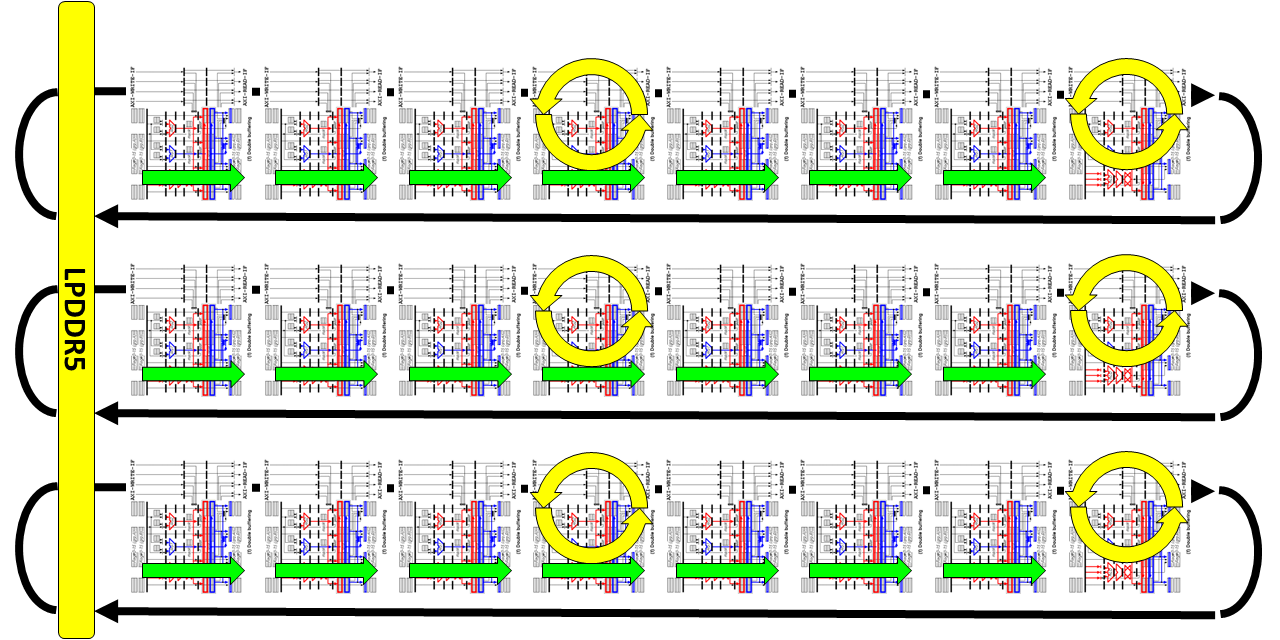
\includegraphics[angle=270,origin=b,width=0.80\textwidth]{fig07.eps}
\caption{\label{fig:micro}Micro pipelining}
\end{figure}

\begin{figure}[htbp]
\center
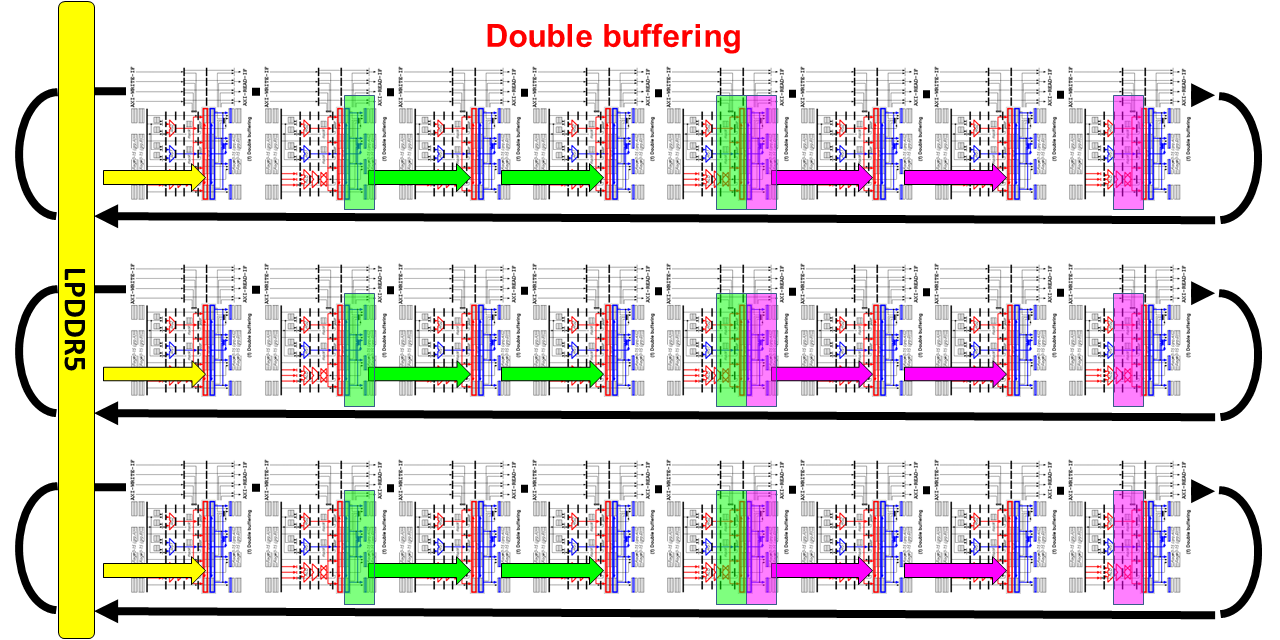
\includegraphics[angle=270,origin=b,width=0.80\textwidth]{fig08.eps}
\caption{\label{fig:medium}Medium pipelining}
\end{figure}

\begin{figure}[htbp]
\center
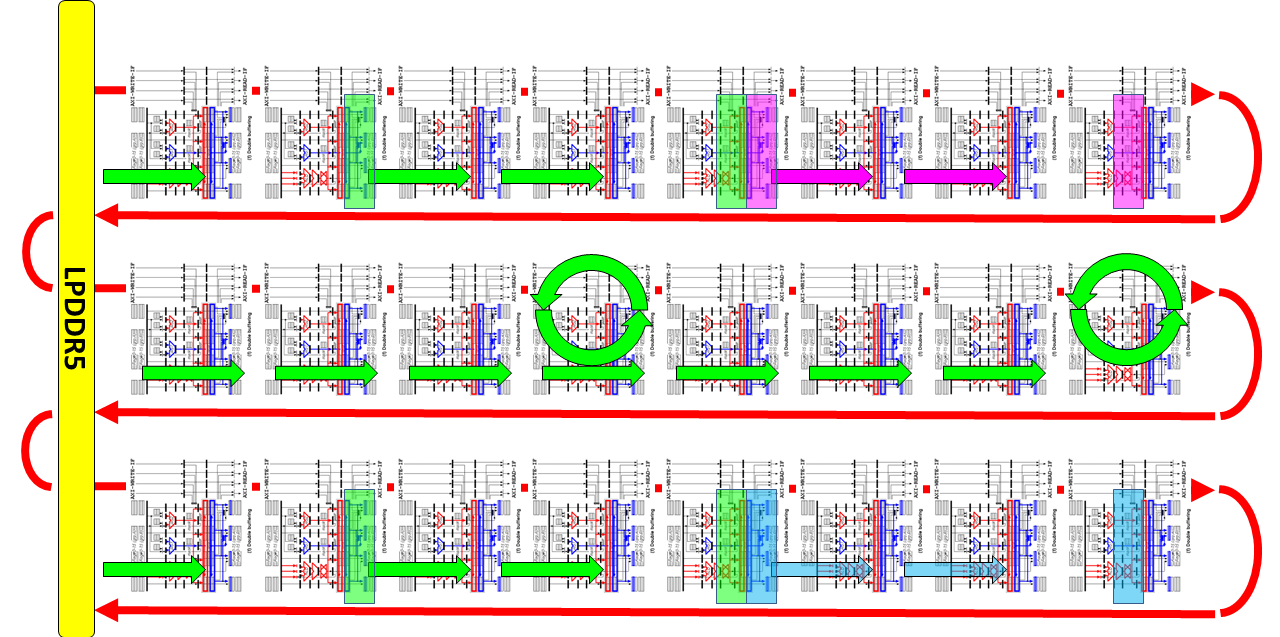
\includegraphics[angle=270,origin=b,width=0.80\textwidth]{fig09.eps}
\caption{\label{fig:macro}Macro pipelining}
\end{figure}

\begin{figure}[htbp]
\center
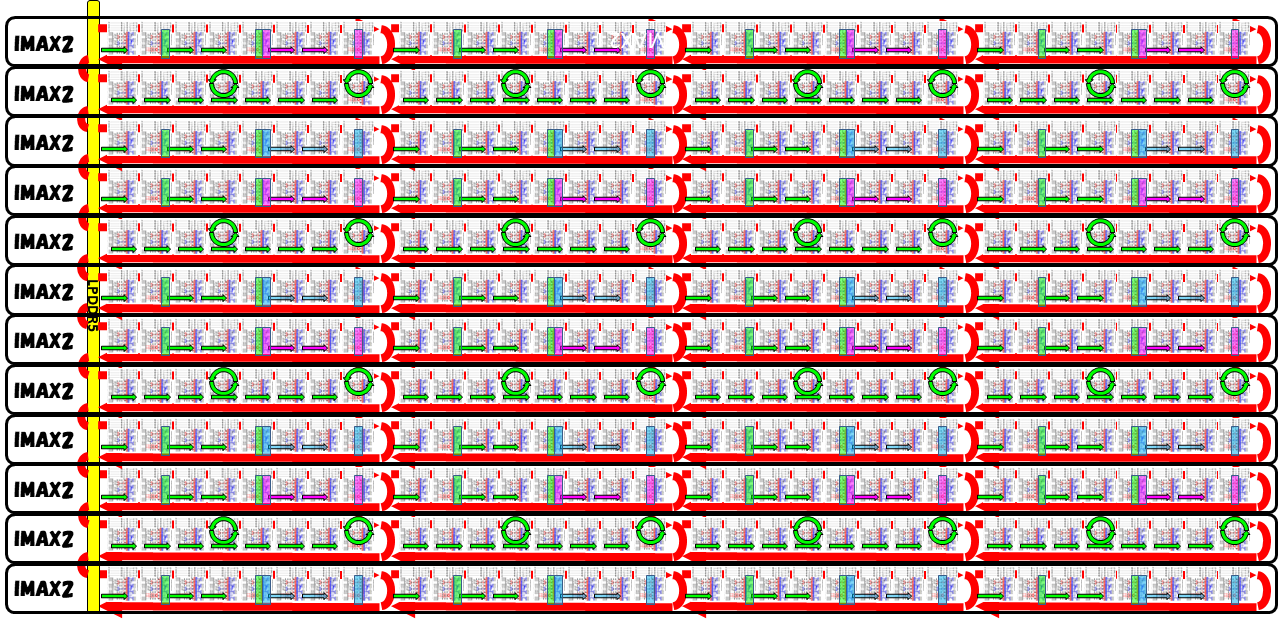
\includegraphics[angle=270,origin=b,width=0.80\textwidth]{fig10.eps}
\caption{\label{fig:all}Multilevel pipelining}
\end{figure}

\begin{figure}[htbp]
\center
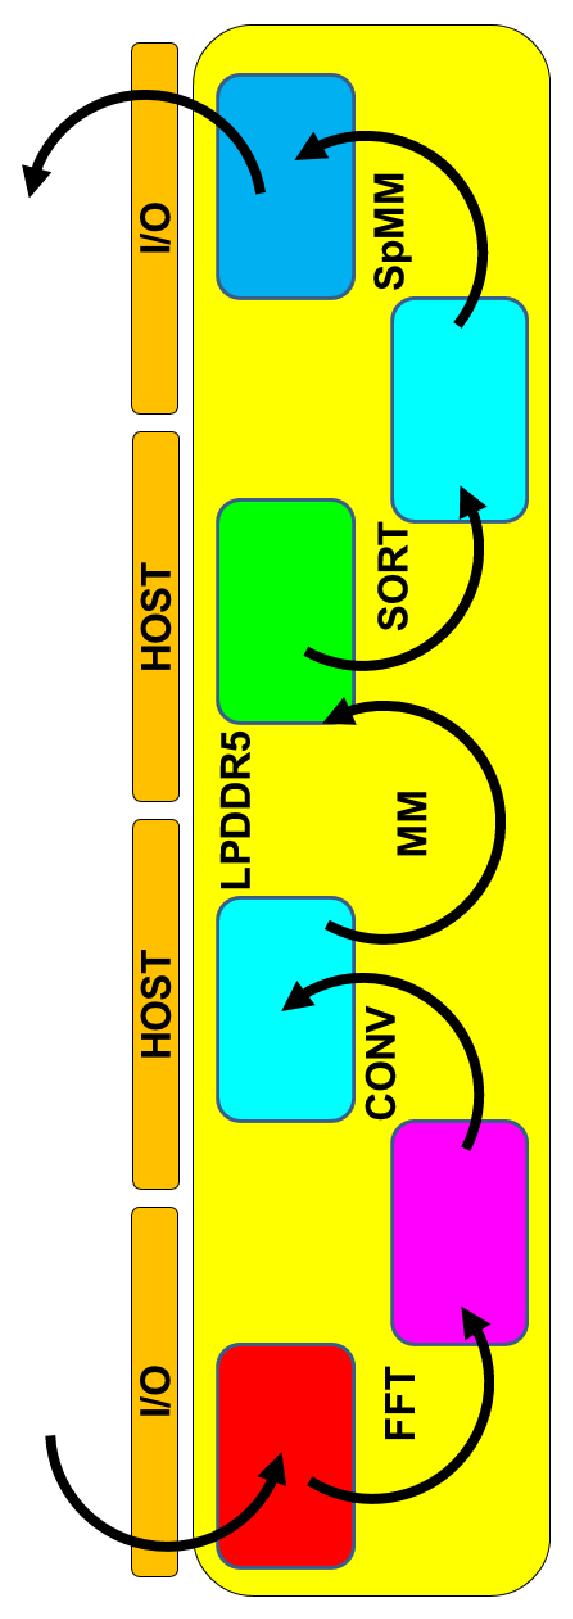
\includegraphics[angle=270,origin=b,width=0.80\textwidth]{fig11.eps}
\caption{\label{fig:map}Mapping of application kernels}
\end{figure}

��\ref{fig:micro}�ϡ�LPDDR5����³���줿ʣ���졼���IMAX2�ȡ��ƥ졼��Υޥ�����
�ѥ��ץ饤��ư��򼨤��Ƥ��롥�ޥ������ѥ��ץ饤��ϡ�CGRA�δ��ܥ⡼�ɤǤ��롥
�ƥ졼��ˤ�ʣ����IMAX2���åפ򥫥���������³�Ǥ��롥���Υ⡼�ɤϡ��������
���ץ�������Ŭ�ѤǤ�������ѥ�����®�Ǥ��롥���ˡ�Figure\ref{fig:medium}
�ϡ�ʣ���졼���IMAX2�ȡ��ƥ졼��Υߥǥ�����ѥ��ץ饤��ư���򼨤��Ƥ��롥
�ߥǥ�����ѥ��ץ饤��ϡ��ƥ졼��ˤ����ơ�����å������Υ��֥�Хåե�
��󥰤ˤ���������Ƥ��ꡤ�����ȡ��ϥå���ؿ�������ӡ�FFT�ʤɡ����ơ���
�֤�ʬΥ��ɬ�פʽ������б����뤳�Ȥ��Ǥ��롥Figure\ref{fig:macro}�ϡ�IMAX3��
�ޥ��� �ѥ��ץ饤��򼨤���ʣ���졼��ϡ�LPDDR5��𤷤ƣ��Ĥ�Ĺ��ʥѥ��ץ饤
��Ȥ���Ϣ�뤵��롥�ƥ졼��ˤϡ��ޥ���������ӥߥǥ�����ѥ��ץ饤�󤬴ޤ�
��롥Figure\ref{fig:all}�ϡ�IMAX3�κǽ����֤򼨤��Ƥ��롥�ƥ졼���ʣ����
IMAX2���åפ���ܤ���Ƥ��롥��\ref{fig:map}�Τ褦�ˡ�¿���Υ졼���CPU����
�����ơ�¿���μ���Υ����ͥ��Ʊ���˥ޥåԥ󥰤��뤳�Ȥ��Ǥ��롥

\begin{figure}[htbp]
\center
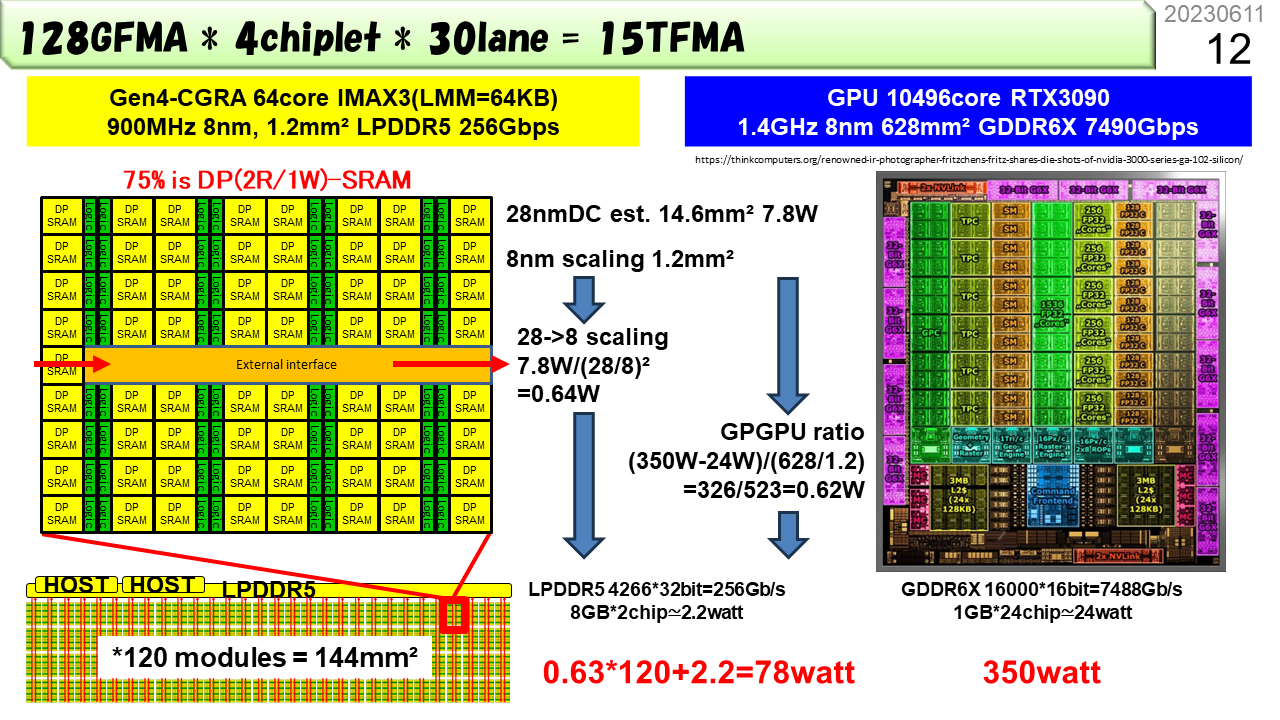
\includegraphics[angle=270,origin=b,width=0.80\textwidth]{fig12.eps}
\caption{\label{fig:chip}Area estimation}
\end{figure}

\clearpage

\section{Prototype}

\begin{figure}[htbp]
\center
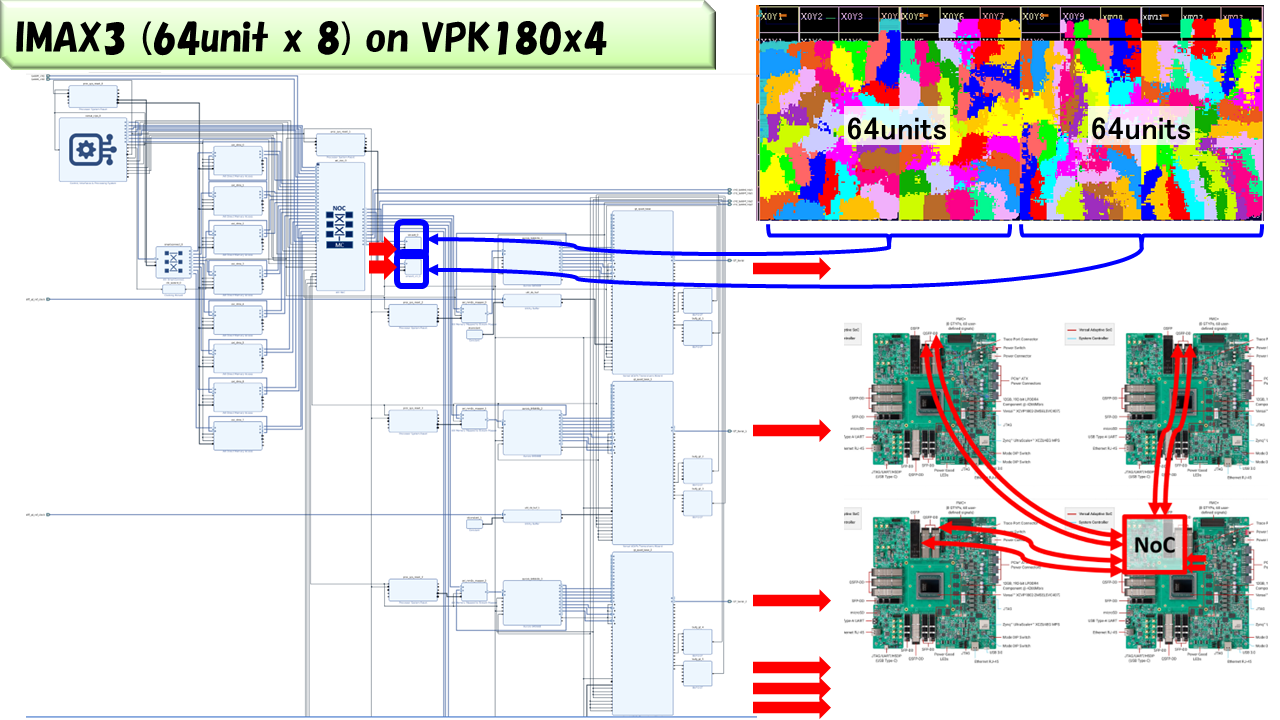
\includegraphics[angle=270,origin=b,width=0.80\textwidth]{fig13.eps}
\caption{\label{fig:proto}Prototype of IMAX3}
\end{figure}

\begin{figure}[htbp]
\center
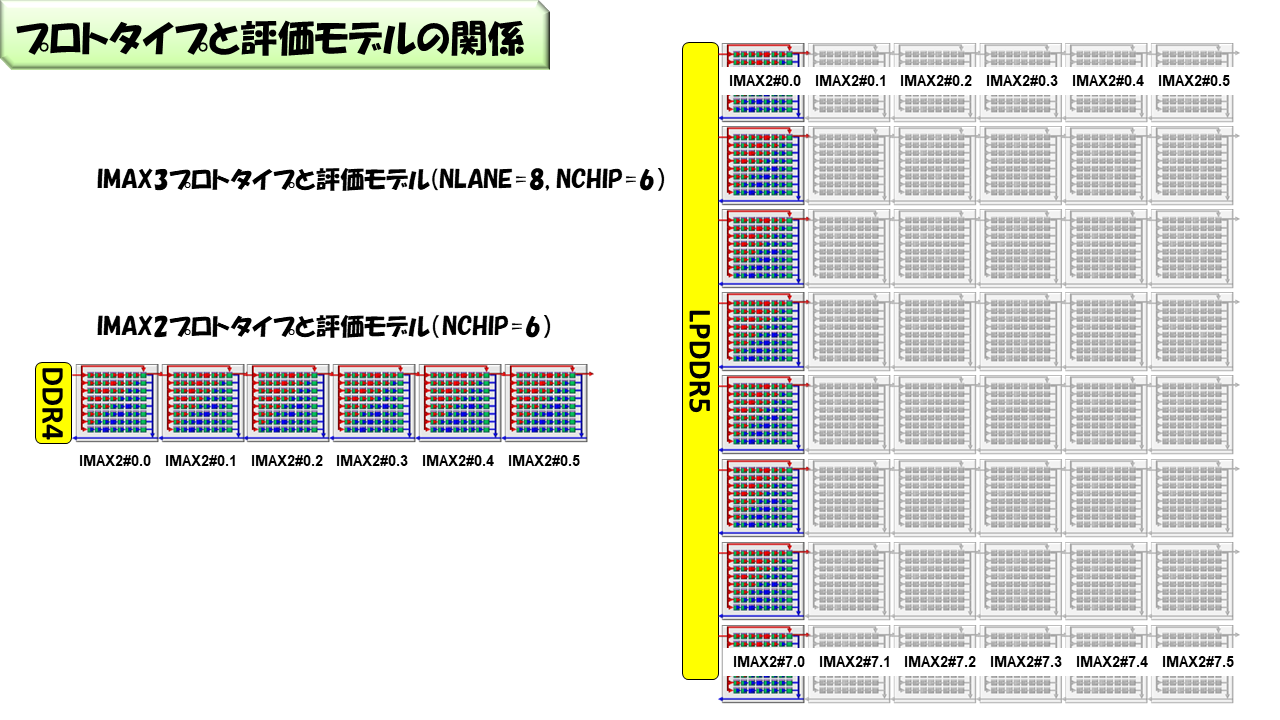
\includegraphics[angle=270,origin=b,width=0.80\textwidth]{fig14.eps}
\caption{\label{fig:evmodel}Evaluation models}
\end{figure}

��\ref{fig:chip}�˼����褦�ˡ�IMAX3��75\%�����Ѥϥ���å������Ǥ��롥
LPDDR5�γƥݡ��Ȥˡ�64��˥åȹ�����IMAX2��4�𥫥���������³������硤10240��
�ڥ졼��������٤˥ޥåԥ󥰤Ǥ��롥LPDDR5�ˤ�����30�ݡ��Ȥ����Ѳ�ǽ�ʾ�硤
307,200���ڥ졼������ޥåԥ󥰤Ǥ��롥8nm���Ѥ���¤������硤144mmʿ���ˡ�
IMAX2��120����ܤǤ��롥Figure\ref{fig:proto}�ϡ�IMAX2��IMAX3�˥������륢��
�פ���ʹ���Υץ��������ȤǤ��롥VPK180�ˤϡ�64��˥åȹ�����IMAX2��2�����
�Ǥ���NoC��𤷤ƹ��8���IMAX2����³�Ǥ��롥��\ref{fig:evmodel}�ϡ��ץ��ȥ�
���פ��Ѥ�����ǽɾ����ǥ�Ǥ��롥���������Τϡ�IMAX2\#0.0��IMAX2\#1.0���ġ�
IMAX2\#7.0��8��Ǥ��롥��IMAX2�ϡ�IMAX2���ץꥱ�������ץ������Ǥϡ�
NLANE=8,NCHIP=1�ι������б����롥������IMAX2���ץꥱ�������ץ������ˤ���
�ơ�NLANE=8,NCHIP=6�ȵ��Ҥ������Ԥ����뤳�Ȥ��ǽ�Ǥ��롥����������ˡ�ϡ���
�������ɹ�����IMAX2��ʣ���졼���������빽�����б����롥����������������Ƥ�
��Τ���Ƭ��IMAX2\#*.0�ΤߤǤ��뤿�ᡤ������������³������³IMAX�μ¹Է��
��0�Ȥʤꡤ�ޤ���������������³��ȼ�������Хإåɤ�¬�ꤵ��ʤ����¹�®�٤ϡ�
�����ޤ������ͤǤ��롥


\chapter{IMAX3 Software}

\section{IMAX3 interface mapped on CPU memory space}

IMAX3�ϡ������̳�������ˡ�IMAX2��ʣ���졼����³���������Ǥ��ꡤ����Τ���
�Υϡ��ɥ��եȥ��󥿥ե������ϡ�IMAX2���Ȥ����楤�󥿥ե������ν���Ǥ��롥

\section{Dataflow example}

\begin{figure}[htbp]
\center
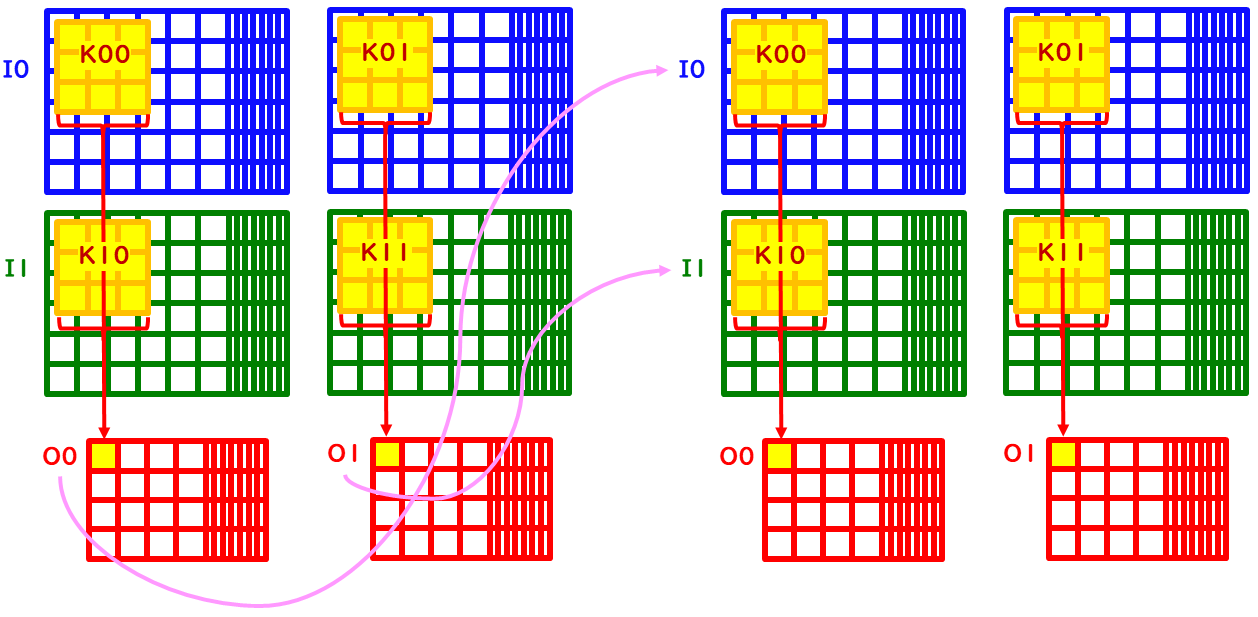
\includegraphics[angle=270,origin=b,width=0.80\textwidth]{fig35.eps}
\caption{\label{fig:4dconv}Tycal series of 4D-array convolution}
\end{figure}

\begin{figure}[htbp]
\center
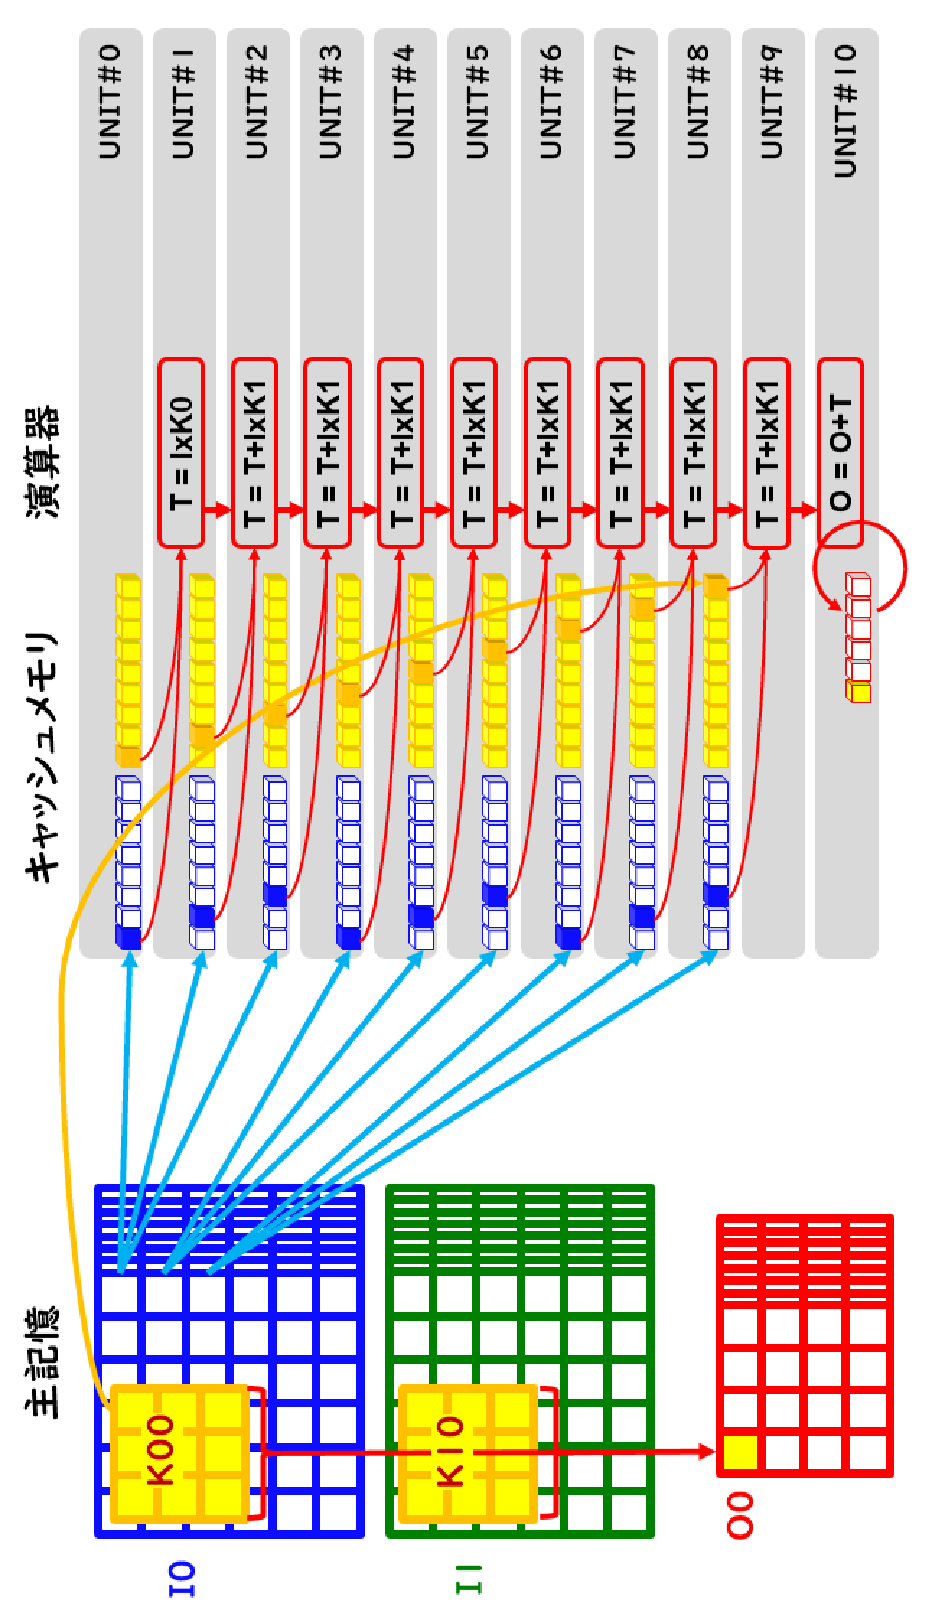
\includegraphics[angle=270,origin=b,width=0.80\textwidth]{fig36.eps}
\caption{\label{fig:4dmap}Typical mappting of convolution}
\end{figure}

\begin{figure}[htbp]
\center
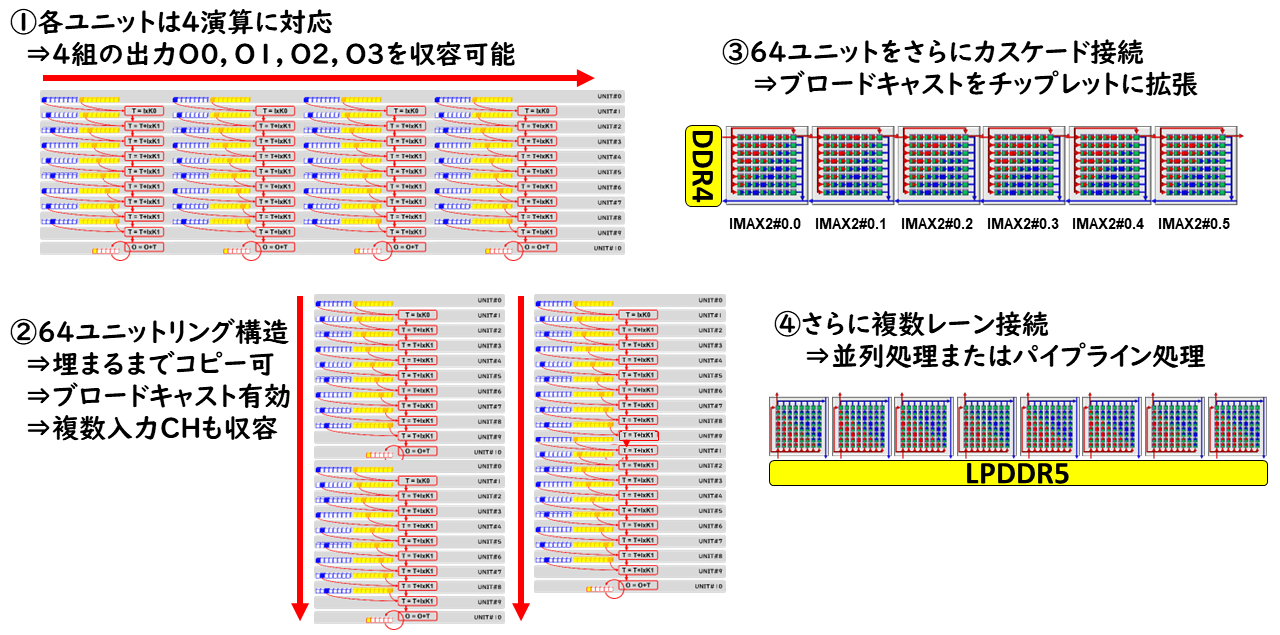
\includegraphics[angle=270,origin=b,width=0.80\textwidth]{fig37.eps}
\caption{\label{fig:options}Several options to speedup convolution}
\end{figure}

\begin{figure}[htbp]
\center
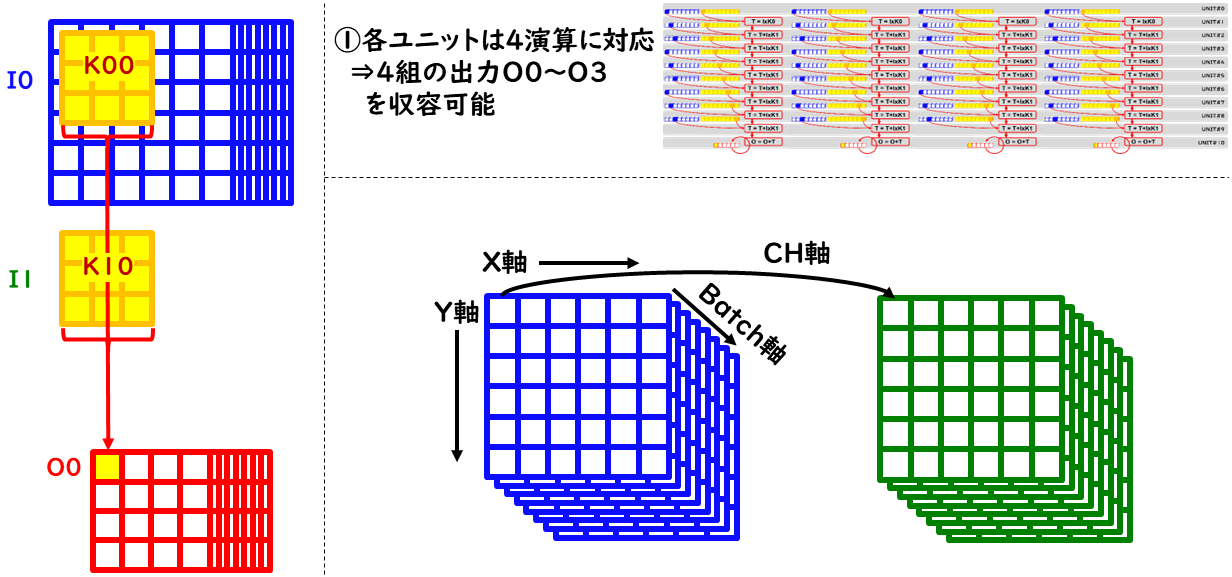
\includegraphics[angle=270,origin=b,width=0.80\textwidth]{fig31.eps}
\caption{\label{fig:twoaxis}Selecting two axis from 4D array}
\end{figure}

\begin{figure}[htbp]
\center
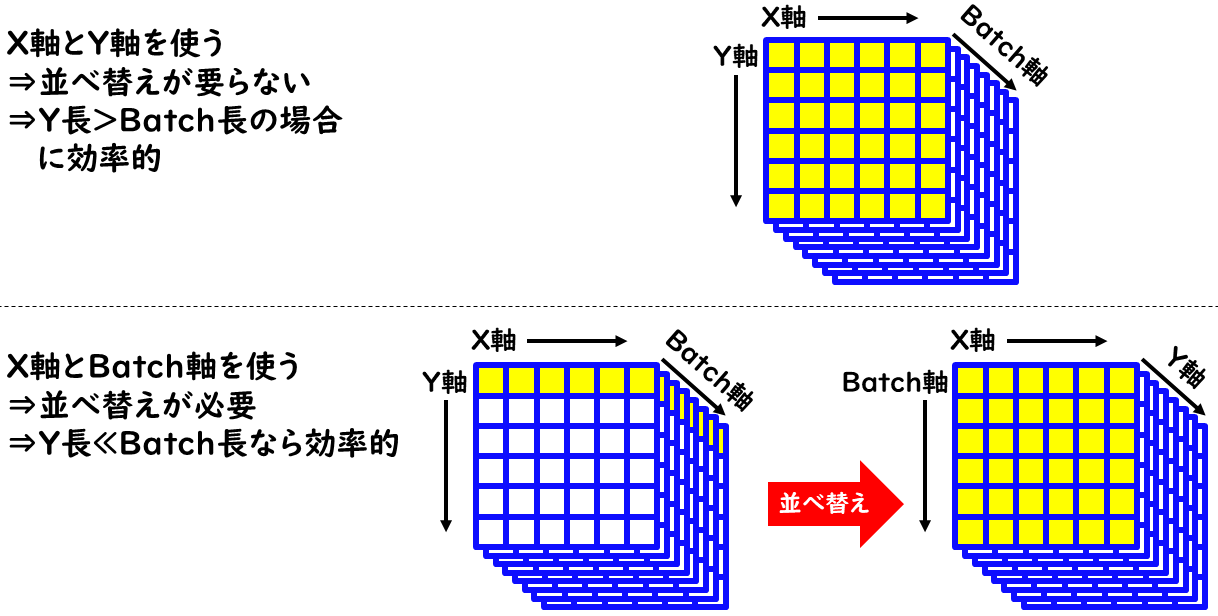
\includegraphics[angle=270,origin=b,width=0.80\textwidth]{fig32.eps}
\caption{\label{fig:optimal}Two options to increase the length of the burst execution}
\end{figure}
 
��\ref{fig:4dconv}�ˡ�ŵ��Ū�ʾ��߹��߱黻�򼨤������ϥǡ���(I)�ΰ����ȡ���
�����륫���ͥ�(K)�ξ軻��Ԥ������¤���롥6x6��2����I0�������������˽Ťʤ�
�Ƥ���Τϡ�6x6�β�����1�ĤΥХå���ʣ����ޤޤ�뤳�Ȥ��б����롥I1��Ʊ�ͤ�
��¤�򤷤Ƥ��ꡤ�㤨�С�I0���Ĥ���ʬ��I1���Ф���ʬ���б����롥���ϥǡ����ȥ���
�ͥ���Ȥ�¿�����ꡤ�����������¤�����O0�Ȥʤ롥���ϥǡ�����2�����Ǥ��ꡤ����
�ͥ�K��X������Y�����ˤ��餷�Ʒ׻��򷫤��֤����ᡤ����O0��2�����Ǥ��롥�ޤ���
���ϥǡ���(I)�Ϥ��Τޤޡ������ͥ�(K)�Τߤ򺹤��ؤ���Ʊ�ͤη׻��򤹤�ȡ��̤�
����O1����ޤ롥���ʤ�������ϥǡ���(I)�������ͥ�(K)�����ϥǡ���(O)�ϡ�����
���4��������Ǥ��롥����ˡ�¿�ؾ��߹��߱黻�Ǥϡ����ϥǡ���(O)�򼡤����ϥǡ�
��(I)�Ȥ��ơ�Ʊ�ͤη׻��򷫤��֤���

�ʾ�ξ��߹��߱黻��IMAX3�ˤ��¹Ԥ�����ˡ�ϡ������Ĥ����롥��
\ref{fig:4dmap}�ϡ�2�������߹��ߤδ��ܷ��Ǥ��롥IMAX�γƥ�˥åȤˤϡ��ۥ���
�Υɥ饤�Ф����椹�륭��å������ȱ黻�郎���äƤ��롥�絭�����Ŀ����ϥǡ�
���ϡ�����å��������Ĥ���ʬ�˥֥����ɥ��㥹�Ȥ��졤�絭���β����Υ�����
��ϡ���������ʬ�˥֥����ɥ��㥹�Ȥ���롥��˥å�0�֤ϡ������ͥ�κ������
������ǡ�������Ф�����˥å�1�֤����롥��˥å�1�֤ϡ��軻��Ԥ�����̤�
��˥å�2�֤����롥�ʾ��Ҥ����Ǹ�ˡ���˥å�10�֤�9�Ĥξ軻��̤����¤���
�����Ϥ�­�����ߡ�3x3�ξ��߹��߱黻��1�Ĵ�λ���롥���ƤΥ�˥åȤ����ϥǡ���
�򱦤˥��եȤ��ʤ��鼡���ȷ׻��������ϥǡ�����Ϣ³���ƹ�������롥�ʾ夬��ŵ
��Ū�ʡ�CGRA�η׻���ˡ�Ǥ��롥

IMAX����ħ�ϡ��ʾ�δ��ܷ���4����������礭���˹�碌���Ȥ߹�碌�뼫ͳ�٤�
¿���ˤ���(��\ref{fig:options})����Ŭ������ɸ�ϡ��¹Ի��֤�û�̤��뤳�ȤǤ�
�ꡤ���ʤϡ��֥����ɥ��㥹�Ȥȡ�����å������κ���º����ѤǤ��롥IMAX2
��1���åפϡ�2�ť롼�פ���٤�Ϣ³�¹ԤǤ���4�Ȥξ��߹��߱黻������Ū��4��
¤�˼����Ǥ��롥�Ĥ�ϡ�4�����ǡ����Τɤμ���2�ť롼�פ˼������뤫�Ǥ��롥��
��I�Τɤμ������֤������ȡ�¾�ϼ�ưŪ�˷�ޤ뤿�ᡤ�ޤ����Ŀ����ϥǡ���
(I)�μ������֡�����ϡ���\ref{fig:twoaxis}�˼�����X����Y�����Хå����������
�뼴��4�ĤǤ��롥��������X���ϡ����ɥ쥹��Ϣ³���뤿�ᡤɬ�����֤٤��Ǥ��롥
Ʊ�ͤˡ�����ͥ뼴�ϡ�64��˥åȤ����뤿������Ѥ���и�Ψ���ɤ����ᡤ�Ĥ�
���ϡ�Y���ޤ��ϥХå�����2��Ȥʤ롥

��\ref{fig:optimal}�ˡ�2�Ĥμ�����ˡ�򼨤���X����Y����Ȥ���硤�����Υǡ���
�ϡ�Ϣ³���ɥ쥹�Ǥ��뤿�ᡤ�¤��ؤ������פǤ��롥X��Ĺ����Y��Ĺ����褸��1
��Υǡ���������������˥å���Υ���å������������硤�Ǥ��Ψ���ɤ���
�㤨�С�����å�����꤬16Kwordʬ����С�128x128�ޤǼ��ƤǤ��롥256x256��
���⡤���η��Τޤޡ�Y�����ˣ�ʬ�䤷�Ƽ¹Ԥ���Ф褤��������¿�ؾ��߹��ߤ�
�����Ǥϡ�2x2���ξ������������ˤʤ뤿�ᡤIMAX��Ϣ³�¹Ի��֤�û���ʤꡤ��ư
�����Хإåɤ��礭���ʤ롥���Τ褦�ʾ�硤Y��������˥Хå�����Ȥ����¤�
�ؤ���ȼ�������Хإåɤ����ä��뤬���Хå�����100�ξ�硤2x100�Ȥʤꡤ�ǡ���
���������礭���Ǥ�����ư�����Хإåɤ�︺�Ǥ��롥3�������߹��ߤξ��⡤Ʊ
�ͤˡ�IMAX��Ϣ³ư����֤�Ĺ��������ư����򸺤餻�Ф褤��

\section{Programming model of Macro pipelining}

\begin{figure}[htbp]
\center
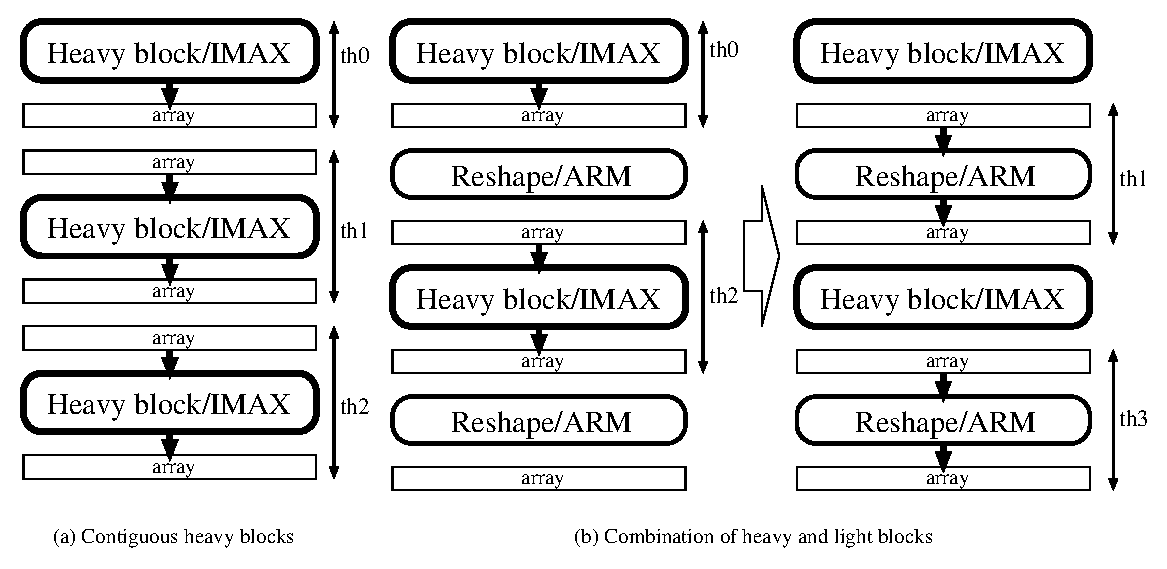
\includegraphics[angle=0,origin=b,width=0.85\textwidth]{macro-pipe.eps}
\caption{\label{fig:model0}Programming model}
\end{figure}

��\ref{fig:model0}�ϡ��ޥ����ѥ��ץ饤�˥󥰤˴ؤ��롤�ץ�����ߥ󥰥�ǥ��
���롥(a)�ϡ��������֤�Ĺ����֤�3�Ĥ��ꡤ3�ĤΥ���åɤ�ư���ơ��ơ���
IMAX�ˤ���®������ޥ����ѥ��ץ饤�˥󥰤Ǥ��롥�ƥ���åɤ����ϤȽ��Ϥ���
�Ĥ��ʤ��褦������åɴ֤Υǡ�����¤�˥��֥�Хåե���ɬ�פȤʤ롥������(b)
�ϡ��������֤�Ĺ����֤�IMAX�ˤ��¹Ԥ����ΤΡ������֤ˡ�����ź����������
�������ۥ��Ȥˤ��û���ֽ�������ߤ��륱�����Ǥ��롥û���ֽ�������֥�Хåե�
�Ȥ������Ѥ��뤳�Ȥˤ�ꡤ���ƤΥ���åɴ֤˥��֥�Хåե���Ŭ�Ѥ��������
�١���������̤������Ǥ��롥

\section{Programming style of Macro pipelining}

\begin{figure}[htbp]
\center
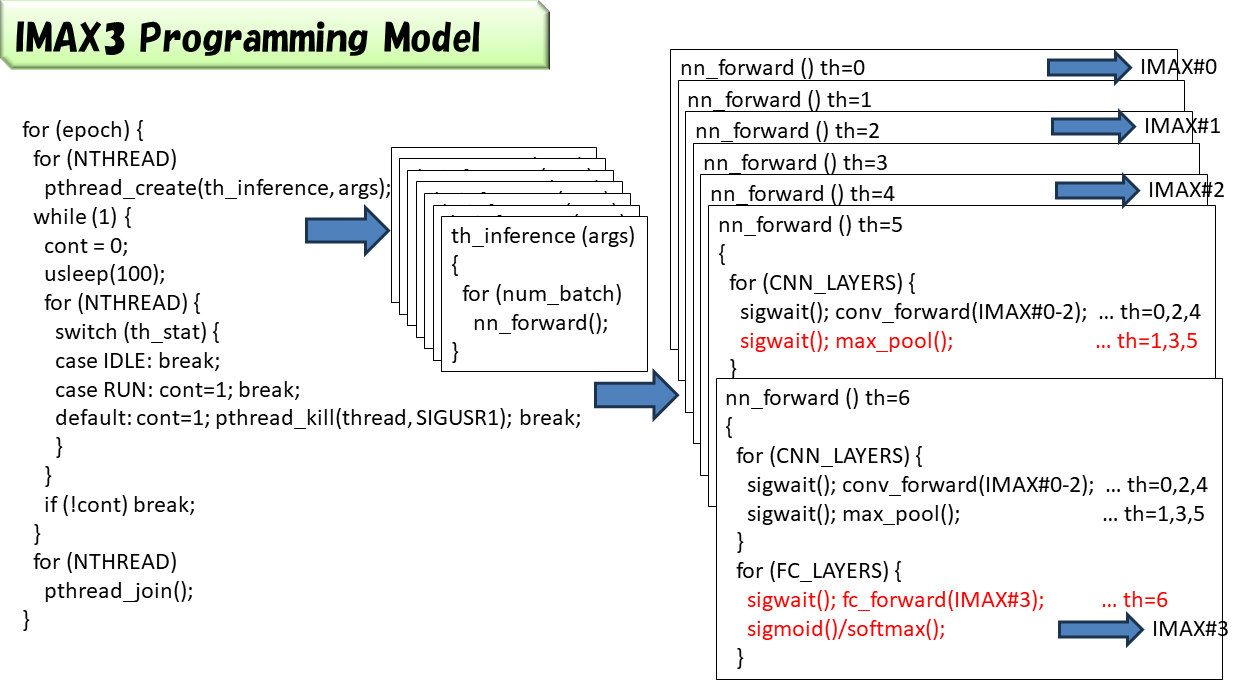
\includegraphics[angle=270,origin=b,width=0.85\textwidth]{fig15.eps}
\caption{\label{fig:model1}Programming stype}
\end{figure}

��\ref{fig:model1}�ϡ��ץ�����ߥ󥰥�������Ǥ��롥�ޥ����ѥ��ץ饤�˥󥰤�
�ϡ�ʣ���Υ���åɤ�ư�����롼�׹�¤�����񤹤�ؿ�(th\_inference)��Ʊ����
�¹Գ��Ϥ��롥th\_inference()�ϡ�¿��CNN�򥷥ߥ�졼�Ȥ���nn\_forward()��
���֤��¹Ԥ��롥nn\_forward()�ϡ�ʣ������åɤˤ��Ʊ���˼¹Ԥ�����ΤΡ�
�ƥ���åɤϡ�ô���ս�Τߤ�¹Ԥ��������ؤȸ����ؤν�����λ�Ȥ��Ԥ���碌��
�Ԥ��Ĥġ��ѥ��ץ饤�������Ԥ������ؤΤ�����LANE������Ȥ���ؿ��ƤӽФ�����
IMAX2����Ѥ��롥�ޥ����ѥ��ץ饤�˥󥰤ˤϡ�HOST��IMAX2���ơ�ʣ�����ä��Ƥ�
�롤Busy loop�ǤϤʤ���sigwait()��Ȥ����Ȥˤ�ꡤHOST�Υ���������ʬ�ˤʤ���
��ˤ⡤����åɴ֤��Ԥ���碌��HOST��ǽ�Ϥ�Ķ���ʤ����ȤߤȤ��Ƥ��롥


\chapter{Examples}

\section{Image recognition (tsim)}

MNIST

\shabox{
\leftline{cent\% make -f Makefile-cent.emax7nc all clean}
\leftline{cent\% cd ../; tsim/tsim-cent.emax7nc -x -t -I0 -C1 -F1}
}

\shabox{
\leftline{acap\% make -f Makefile-acap.emax7+dma all clean}
\leftline{acap\% cd ../; tsim/tsim-acap.emax7+dma -x -t -I0 -C1 -F1}
}

\vskip .1in

CIFAR10

\shabox{
\leftline{cent\% make -f Makefile-cent.emax7nc all clean}
\leftline{cent\% cd ../; tsim/tsim-cent.emax7nc -x -t -I1 -C6 -F2}
}

\shabox{
\leftline{acap\% make -f Makefile-acap.emax7+dma all clean}
\leftline{acap\% cd ../; tsim/tsim-acap.emax7+dma -x -t -I1 -C6 -F2}
}

\begin{figure}[htbp]
\center
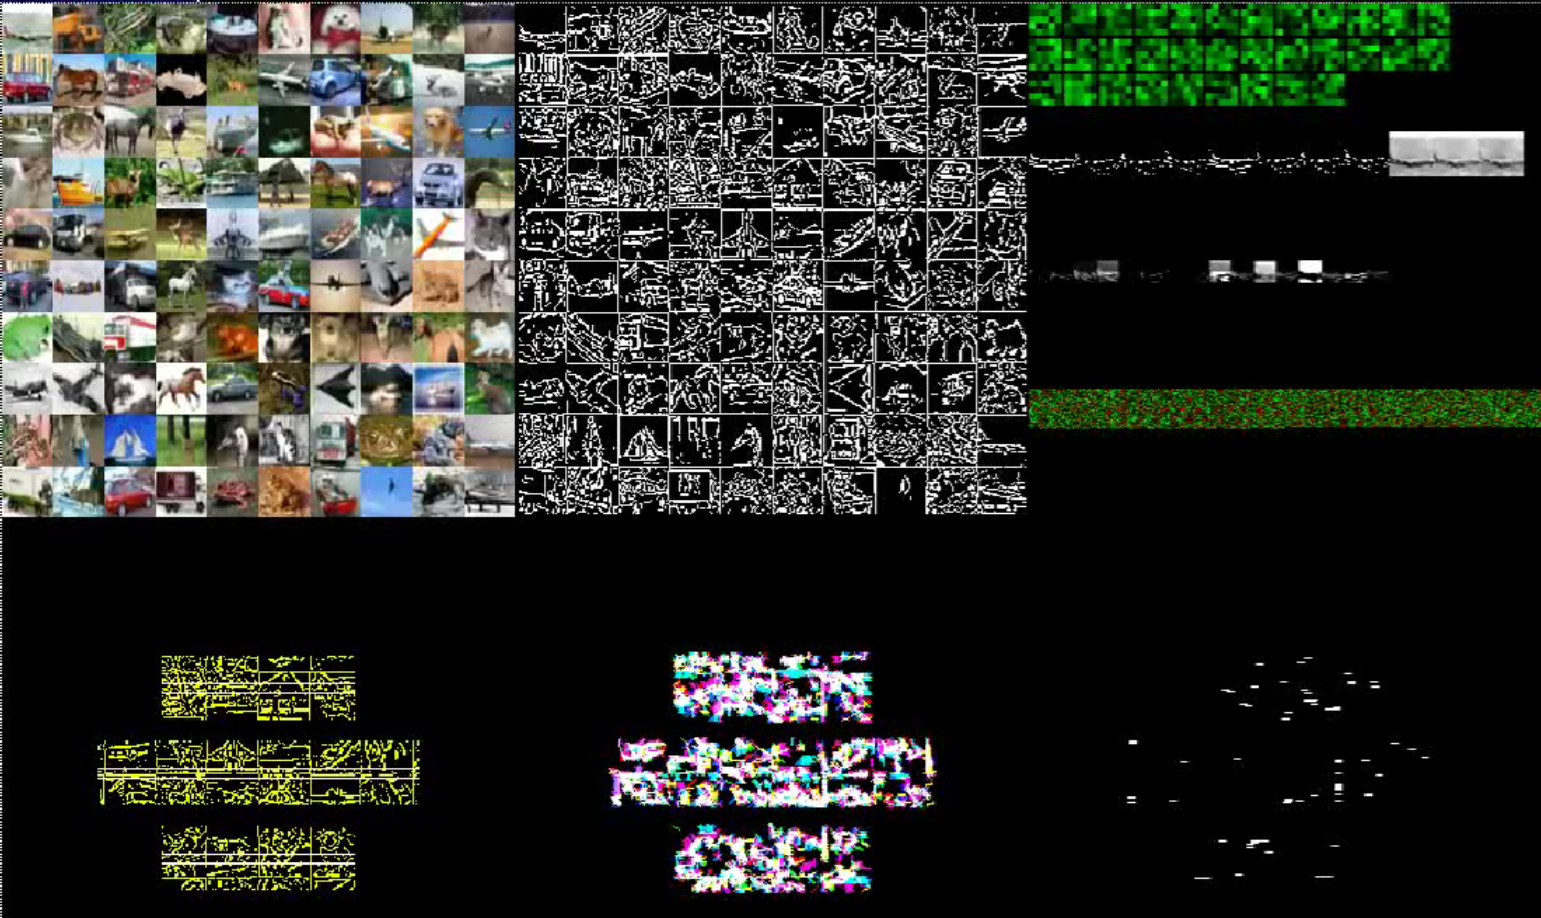
\includegraphics[angle=270,origin=b,width=0.80\textwidth]{ssim.eps}
\caption{Image recognition (training + inference)}
\end{figure}

\clearpage

\subsection{Header}

IMAX3�ϡ�ʣ����IMAX2�졼������椹�뤿��ˡ�ARM�Υޥ������åǥ��󥰤�����
���롥NTHREAD�ϡ�ʣ��IMAX2�졼��ε�ư�˺ݤ���ARM�ˤ����Ƶ�ư���Ƥ��������
�ɿ��Ǥ��롥EMAX\_LANE�ϡ�Ʊ���˵�ư����IMAX2�졼������椹�뤿��Ρ�������
�����åȤξ�¤Ǥ��롥�ޤ���NLANE�ϡ��µ��ˤ����Ƹ��Ф��줿IMAX2�Υ졼�����
���롥EMAX\_LANE��Ķ���ơ��µ��ˤ����Ƹ��Ф��줿IMAX2�ϡ����Ѥ���ʤ�������
�����NLANE�˥��åȤ�����ͤϡ�ɬ����EMAX\_LANE�ʲ��Ǥ��롥�ʤ���NTHREAD�ϡ�
NLANE�ʾ�Ǥʤ���Фʤ�ʤ���

\begin{screen}
\scriptsize
\begin{verbatim}
#define MAX_NTHREAD 16
volatile struct th_inference_args {
  int      thid;
  int      stat;     /* 0:idle, 1:run, 2:wait (enq/deq, DMA, EXEC) */
  sigset_t sigset;   /* sys/_sigset.h 2B/4B */
  int      deq;
  int      enq;
  float4D *slice;
  CNNet   *net;
  int      batch_size;
  int      nchan;
  int      insize;
} th_inference_args[MAX_NTHREAD];
volatile int th_inference_retv[MAX_NTHREAD];
pthread_t    th_inference_t[MAX_NTHREAD];
void         th_inference(struct th_inference_args *);
\end{verbatim}
\end{screen}

\subsection{IMAX3 thread driver}

ʣ����IMAX2��ư���ơ��ޥ����ѥ��ץ饤���������ݤˤϡ�IMAX2�����ͥ���
��ؿ���åѡ��ʰʲ�����Ǥ�th\_inference�ˤ��Ѱդ���ARM��pthread\_create����
���ơ�NTHREAD�ĤΥ���åɤ�ư���롥����åɤΰ����ϡ�thread�ֹ桤�ѥ��ץ�
����Ʊ���Ѥ�enq/deq��ޤࡥ

\begin{screen}
\scriptsize
\begin{verbatim}
  int THREAD;
  for (THREAD=0; THREAD<NTHREAD; THREAD++) {
    th_inference_args[THREAD].thid       = THREAD;
    th_inference_args[THREAD].stat       = 1; /* run */
    sigemptyset(&th_inference_args[THREAD].sigset);
    sigaddset(&th_inference_args[THREAD].sigset, SIGUSR1);
    pthread_sigmask(SIG_BLOCK, &th_inference_args[THREAD].sigset, NULL);
    th_inference_args[THREAD].enq        = 0;
    th_inference_args[THREAD].deq        = 0;
    th_inference_args[THREAD].slice      = &slice;
    th_inference_args[THREAD].net        = net;
    th_inference_args[THREAD].batch_size = batch_size;
    th_inference_args[THREAD].nchan      = nchan;
    th_inference_args[THREAD].insize     = insize;
  }
  if (NTHREAD > 1) {
    for (THREAD=0; THREAD<NTHREAD; THREAD++)
      pthread_create(&th_inference_t[THREAD], NULL, (void*)th_inference, &th_inference_args[THREAD]); /* 0-(NTHREAD-1) */
    while (1) {
      int cont = 0;
      usleep(4000); /* 4msec 2024/01/24 Nakashima */
      for (THREAD=0; THREAD<NTHREAD; THREAD++) {
        switch (th_inference_args[THREAD].stat) {
        case 0:            break;/* idle */
        case 1:  cont = 1; break;/* run */
        default: cont = 1; pthread_kill(th_inference_t[THREAD], SIGUSR1); break; /* wait */
        }
      }
      if (!cont) break;
    }
    for (THREAD=0; THREAD<NTHREAD; THREAD++)
      pthread_join(th_inference_t[THREAD], NULL);
  }
  else {
    for (THREAD=0; THREAD<NTHREAD; THREAD++)
      th_inference(&th_inference_args[THREAD]);
  }
\end{verbatim}
\end{screen}

\clearpage

\subsection{IMAX3 thread wrapper}

��åѡ��ϡ�ʣ��Ʊ���˵�ư����롥������ʣ������åɤ��ѥ��ץ饤��ư����
����������Ϳ�����륹��å��ֹ�˴�Ť���ô���ս��¹Ԥ���褦���Ҥ��롥

\begin{screen}
\scriptsize
\begin{verbatim}
/* IMAX3 MACROPIPELIING for EVALUATION */
void th_inference(struct th_inference_args *args)
{
  int THREAD     = args->thid;
  float4D *slice = args->slice;
  CNNet *net     = args->net;
  int batch_size = args->batch_size;
  int nchan      = args->nchan;
  int insize     = args->insize;
  int j, k;
  /************************************/
  /* TARGET of MACRO-PIPELINING/IMAX3 */
  /************************************/
  slice->nstrides = batch_size;
  slice->nchannel = xtest.nchannel;
  slice->kstrides = xtest.kstrides;
  slice->stride_size = xtest.stride_size;
  for (j=0; j+batch_size<=xtest.nstrides; j+=batch_size) {
    if (THREAD == 0) {
      slice->data = &(xtest.data[j*xtest.stride_size*xtest.kstrides*xtest.nchannel]);
      if (cnn_mode) {
        if (enable_x11) {
          F4i2Ipl(batch_size, nchan, insize, insize, I, slice); /* 100batch x 28x28 x 1chan */
          copy_I_to_BGR(D, batch_size, insize, insize, I);
          BGR_to_X(0, D);
        }
        // copy data to input layer
        copy4D(&(net->ninput), slice);
        if (attn_mode) {
          attention(&(net->ninput), &(net->work), &(net->attention)); /* batch,RGB,H,W */
          if (enable_x11) {
            F4i2Ipl(batch_size, nchan, insize, insize, I, &(net->work)); /* 100batch x 28x28 x 1chan */
            copy_I_to_BGR(D, batch_size, insize, insize, I);
            BGR_to_X(3, D);
            F4i2Ipl(batch_size, nchan, insize, insize, I, &(net->ninput)); /* 100batch x 28x28 x 1chan */
            copy_I_to_BGR(D, batch_size, insize, insize, I);
            BGR_to_X(1, D);
          }
        }
      }
      if (eye_mode) {
        F4i2Ipl(batch_size, nchan, insize, insize, I, slice); /* 100batch x 28x28 x 1chan */
        copy_I_to_BGR(R, batch_size, insize, insize, I); /* R <- I */
        copy_I_to_BGR(L, batch_size, insize, insize, I); /* L <- I */
        if (enable_x11)
          BGR_to_X(0, R);
        /* pre-processing by eye-model */
        eyemodel(enable_x11, slit_type); /* L+R -> Sl+Sr */
        /* import Sr to hidden_layer */
        Ipl2F4h(10, WD, HT, Sr, Cr, R, &net->nhidden[0]); /* 100batch x 24x24 x 9chan -> hidden */
      }
    }
    nn_forward(/*MACROPIPE*/1, THREAD, net, c[input_type], f[input_type], &pred, spike_mode);
    if ((NTHREAD==1 || eye_mode)
      ||(CNN_DEPTH==1 && THREAD==2)
      ||(CNN_DEPTH==3 && THREAD==6)
      ||(CNN_DEPTH==4 && THREAD==8)
      ||(CNN_DEPTH==6 && THREAD==12)) {

      for (k=0;k<batch_size;k++) {
        float *A = &(pred.data[k*pred.stride_size]);
        nerr += (MaxIndex(A, pred.stride_size) != ytest[j+k]);
      }
      if (enable_x11) {
        clear_BGR(D);
        copy_H_to_BGR(D+WD*(HT*1/4), &net->nhidden[0]);
        copy_H_to_BGR(D+WD*(HT*2/4), &net->nhidden[CNN_DEPTH-1]);
        BGR_to_X(2, D);
        while (x11_checkevent());
      }
    }
  }
  /*********************************/
  /* END of MACRO-PIPELINING/IMAX3 */
  /*********************************/
  args->stat = 0; /* idle */
}
\end{verbatim}
\end{screen}

\clearpage

\subsection{IMAX3 region}

�ʲ���nn\_forward�ϡ�����ե���󥹤�Ԥ��Ǿ�̴ؿ��Ǥ��롥���ߤϡ����Ȥ�
��ꡤ����THREAD�ȡ����Ѥ���IMAX2�졼���ֹ���Ϣ�դ��Ƥ��롥�ޤ���enq/deq��
�Ѥ��ơ��ޥ����ѥ��ץ饤���Ʊ�����Ƥ��롥���衤��ư���ġ��뤬��������С���
��Ȥ����פȤʤ롥

\begin{screen}
\scriptsize
\begin{verbatim}
void nn_forward(int MACROPIPE, int THREAD, CNNet *net, struct c *c, struct f *f, float2D *oubatch, int spike_mode)
{ /* NTHREAD 1:MACRO_PIPE_OFF 2-:MACRO_PIPE_ON */
  /*                             EMAX7:NTHREAD=8 other:NTHREAD=1 */
  /*                              ZYNQ:NLANE=X                   */
  /*                              othr:NLANE=4                   */
  /* train:     nn_forward(0, 1)                                 */
  /* inference: nn_forward(1, T)                                 */
  /* camera:    nn_forward(0, 1)                                 */
  /* th#>0�ξ��,����enq==deq�ʤ��Ե� �ǽ�th#̤���ξ��,����enq!=deq�ʤ��Ե� */
  /* �Ե����֤ˤʤ����,����deq=1-deq�˹���                                  */
  /* ����enq�Ǽ��Ȥ�dbuf����                                                 */
  /* �Ǹ��,            ����enq=1-enq�˹���                                  */
  /* DBUF��                                                              */
  /* th#0      ****0* ****1* ****2*  CNN0:ninput->nhidden[0]                 */
  /*      enq 0     11     00     11                                         */
  /*      deq 0     01     10     01                                         */
  /* th#1     -------*0*    *1*    *2*  nhidden[0]->npool[0]                 */
  /*      enq 0        11     00     11                                      */
  /*      deq 0        01     10     01                                      */
  /* th#2     ----------****0* ****1* ****2*  CNN1:npool[0]->nhidden[1]      */
  /*      enq 0              11     00     11                                */
  /*      deq 0              01     10     01                                */
  /* th#3     ----------------*0*    *1*    *2*  nhidden[1]->npool[1]        */

  /* NHIDDEN/NPOOL��DBUF�Ȥ��ƻȤ����                                       */
  /* th#0      ****0*  ****1*  ****2*  CNN0:ninput->nhidden[0]               */
  /*      enq 0     1 1     0 0     1 1                                      */
  /*      deq 0     0 1     1 0     0 1                                      */
  /* th#1     ------*0*     *1*     *2*  nhidden[0]->npool[0]                */
  /*      enq 0       1     1 0     0 1                                      */
  /*      deq 0       0     1 1     0 0     1                                */
  /* th#2     ---------****0*  ****1*  ****2*  CNN1:npool[0]->nhidden[1]     */
  /*      enq 0             1 1     0 0     1 1                              */
  /*      deq 0             0 1     1 0     0 1                              */
  /* th#3     --------------*0*     *1*     *2*  nhidden[1]->npool[1]        */

  int batch_size = net->ninput.nstrides;
  int i, j, k, l;
  float *temp;

  if (cnn_mode && !(CNN_DEPTH==1 && FC_DEPTH==1) && !(CNN_DEPTH==3 && FC_DEPTH==1)
               && !(CNN_DEPTH==4 && FC_DEPTH==1) && !(CNN_DEPTH==6 && FC_DEPTH==2)) { /* IGNORE MACRO_PIPE in cnn_mode */
    if (THREAD > 0) exit(0);
  }
  if (eye_mode) { /* IGNORE MACRO_PIPE in eye_mode */
    if (THREAD > 0) exit(0);
  }
  if (spike_mode) { /* IGNORE MACRO_PIPE in spike_mode */
    if (THREAD > 0) exit(0);
  }
  if (spike_mode) {
    /* SMAX1 assumes -V* -C1 */
    // add bias broadcast<2>(hbias, hidden.shape);
    temp = net->nhidden[0].data;
    for (i=0;i<net->nhidden[0].nstrides;i++) {
      for (j=0;j<net->nhidden[0].nchannel;j++) {
        for (k=0;k<net->nhidden[0].kstrides*net->nhidden[0].stride_size;k++,temp++)
          *temp += net->hbias[0].data[j];
      }
    }
    relu4(&(net->nhidden[0]));                                                 /* V1->c.nhidden[0].data */
    max_pooling(&(net->npool[0]), &(net->nhidden[0]), c[0].psize, c[0].psize); /*   ->c.npool[0].data */
    flat4Dto2D(&(net->nflat[0]), &(net->npool[0]));                            /*   ->f.nflat[0].data */
    smax_trial(0, net, c, f); /* IGNORE MACRO_PIPE */
  }
\end{verbatim}
\end{screen}

\begin{screen}
\scriptsize
\begin{verbatim}
  else {
    int LANE = 0;
    for (l=0; l<CNN_DEPTH; l++) {
      /***************************************************************************/
      if (!MACROPIPE || NTHREAD==1 || eye_mode) {}
      else if (THREAD == l*2) {
        if (THREAD>0) while (th_inference_args[THREAD-1].enq==th_inference_args[THREAD-1].deq) { inference_sigwait; }
                      while (th_inference_args[THREAD  ].enq!=th_inference_args[THREAD  ].deq) { inference_sigwait; }
        //th_inference_args[THREAD-1].deq = 1-th_inference_args[THREAD-1].deq; /* DBUF�� */
#if defined(EMAX7)
        if (l >= NLANE) {
          printf("nn_forward_CNN: LANE(%d) >= NLANE(%d)\n", l, NLANE);
          exit(1);
        }
        LANE = l;
        emax7[LANE].sigwait = 1; /* ON */
        emax7[LANE].sigstat = &th_inference_args[THREAD].stat;
        emax7[LANE].sigset  = &th_inference_args[THREAD].sigset;
#endif
      }
      else
        goto end_of_cnn; /* skip other task */
      /***************************************************************************/
      if (l>0 || cnn_mode) {
        // first layer, conv, use stride=2
        /***********************ninput*** V CNN    */
#ifndef CUDA
/*��IMAX3��*/conv_forward(THREAD, LANE, l==0?&(net->ninput):&(net->npool[l-1]), &(net->Ki2h[l]),
                          &(net->nhidden[l]), c[l].ksize, &(net->tmp_col[l]), &(net->tmp_dst[l]));
#else
        conv_forward_cuda(l==0?&(net->ninput):&(net->npool[l-1]), &(net->Ki2h[l]),
                          &(net->nhidden[l]), c[l].ksize, &(net->tmp_col[l]), &(net->tmp_dst[l]));
#endif
      }

      // add bias broadcast<2>(hbias, hidden.shape);
      temp = net->nhidden[l].data;
      for (i=0;i<net->nhidden[l].nstrides;i++) {
        for (j=0;j<net->nhidden[l].nchannel;j++) {
          for (k=0;k<net->nhidden[l].kstrides*net->nhidden[l].stride_size;k++,temp++)
            *temp += net->hbias[l].data[j];
        }
      }
      // Activation, relu, backup activation in nhidden
      // nhidden = F<relu>(nhidden);
      relu4(&(net->nhidden[l]));
      copy4D(&(net->nhiddenbak[l]), &(net->nhidden[l]));

      /***************************************************************************/
      if (!MACROPIPE || NTHREAD==1 || eye_mode) {
      }
      else if (THREAD == l*2) {
        if (THREAD>0) th_inference_args[THREAD-1].deq = 1-th_inference_args[THREAD-1].deq;
                      th_inference_args[THREAD  ].enq = 1-th_inference_args[THREAD  ].enq;
      }
      /***************************************************************************/
    end_of_cnn:
\end{verbatim}
\end{screen}

\begin{screen}
\scriptsize
\begin{verbatim}
      /***************************************************************************/
      if (!MACROPIPE || NTHREAD==1 || eye_mode) {
      }
      else if (THREAD == l*2+1) {
        while (th_inference_args[THREAD-1].enq==th_inference_args[THREAD-1].deq) { inference_sigwait; }
        while (th_inference_args[THREAD  ].enq!=th_inference_args[THREAD  ].deq) { inference_sigwait; }
        //th_inference_args[THREAD-1].deq = 1-th_inference_args[THREAD-1].deq; /* DBUF�� */
      }
      else
        goto end_of_maxpool; /* skip other task */
      /***************************************************************************/

      // max pooling /*����nhidden���������鳫��*/
      max_pooling(&(net->npool[l]), &(net->nhidden[l]), c[l].psize, c[l].psize);
      copy4D(&(net->npoolbak[l]), &(net->npool[l]));

      /***************************************************************************/
      if (!MACROPIPE || NTHREAD==1 || eye_mode) {
      }
      else if (THREAD == l*2+1) {
        th_inference_args[THREAD-1].deq = 1-th_inference_args[THREAD-1].deq; /* NHIDDEN/NPOOL��Ȥä�DBUF�ξ�� */
        th_inference_args[THREAD  ].enq = 1-th_inference_args[THREAD  ].enq;
      }
      /***************************************************************************/
    end_of_maxpool:
      continue;
    }
\end{verbatim}
\end{screen}

\begin{screen}
\scriptsize
\begin{verbatim}
    /***************************************************************************/
    if (!MACROPIPE || NTHREAD==1 || eye_mode)
      LANE = 0;
    else if (THREAD == CNN_DEPTH*2) {
      while (th_inference_args[THREAD-1].enq==th_inference_args[THREAD-1].deq) { inference_sigwait; }
      //th_inference_args[THREAD-1].deq = 1-th_inference_args[THREAD-1].deq; /* DBUF�� */
#if defined(EMAX7)
      if (CNN_DEPTH >= NLANE) {
        printf("nn_forward_FC: CNN_DEPTH(%d) >= NLANE(%d)\n", CNN_DEPTH, NLANE);
        exit(1);
      }
      LANE = CNN_DEPTH;
      emax7[LANE].sigwait = 1; /* ON */
      emax7[LANE].sigstat = &th_inference_args[THREAD].stat;
      emax7[LANE].sigset  = &th_inference_args[THREAD].sigset;
#endif
    }
    else
      goto end_of_fc; /* skip other task */
    /***************************************************************************/
    for (l=0; l<FC_DEPTH; l++) {
      if (l==0)                                                  /***********************npool**** A CNN    */
        flat4Dto2D(&(net->nflat[0]), &(net->npool[CNN_DEPTH-1]));/*************************|****** BOUNDARY */
      else                                                       /***********************nflat**** V FC     */
        copy2D(&(net->nflat[l]), &(net->nout[l-1]));

      // second layer full-connection
/*��IMAX3��*/multiply_float2D(THREAD, LANE, &(net->nout[l]), &(net->nflat[l]), 0, &(net->Wh2o[l]), 0);
      repmat_add(&(net->nout[l]), &(net->obias[l]), batch_size);

      if (l < FC_DEPTH-1) {
        // activation, sigmloid, backup activation in fhidden
#if 1
        sigmoid(&(net->nout[l]));
#else
        relu2(&(net->nout[l]));
#endif
        copy2D(&(net->noutbak[l]), &(net->nout[l]));
      }
      else { /* l == FC_DEPTH-1 */
        // softmax calculation
        softmax2D(&(net->nout[FC_DEPTH-1]), &(net->nout[FC_DEPTH-1]));
      }
    }
    /***************************************************************************/
    if (!MACROPIPE || NTHREAD==1 || eye_mode)   {
    }
    else if (THREAD == CNN_DEPTH*2)
      th_inference_args[THREAD-1].deq = 1-th_inference_args[THREAD-1].deq; /* NHIDDEN/NPOOL��Ȥä�DBUF�ξ�� */
    /***************************************************************************/
    end_of_fc:;
  }

  if ((!MACROPIPE || NTHREAD==1 || eye_mode)
    ||(CNN_DEPTH==1 && THREAD==2)
    ||(CNN_DEPTH==3 && THREAD==6)
    ||(CNN_DEPTH==4 && THREAD==8)
    ||(CNN_DEPTH==6 && THREAD==12)
      ) {
    // copy result out
    copy2D( oubatch, &(net->nout[FC_DEPTH-1]));
  }
}
\end{verbatim}
\end{screen}

%%


\chapter{Appendix}

\section{References}

�ܾϤǤϡ���Ϣ���ͽ񡦵��ʡ�����ʸ������Ϣ�������ץ�����ࡤ����ӡ��ġ�
������������󤹤롥

\begin{itemize}
\parskip 0pc \itemsep 0pc
\item EMAX5�����õ�                                                \dotfill proj-arm64/doc/pat35.tgz
\item IMAX�����õ�                                                 \dotfill proj-arm64/doc/pat36.tgz
\parskip 0pc \itemsep 0pc
\item ARMv8�������ƥ�������ͽ�                                    \dotfill proj-arm64/doc/arm/DDI0487A\_f\_armv8\_arm.pdf
\item ARM Cortex-A53 MPCore Processor Technical Reference Manual\\ \dotfill proj-arm64/doc/arm/ARM-CORTEX-A53\_R0P4.pdf
\item ZYNQ Ultrascale+ SoC Technical Reference Manual\\            \dotfill proj-board/zcu102/doc/ug1085-zynq-ultrascale-trm.pdf
\item AMBA AXI4 and ACE Protocol Specification                     \dotfill proj-arm64/doc/arm/AXI4\_specification.pdf
\item IMAX3 ���ͽ�                                                 \dotfill proj-arm64/doc/emax7/emax7j.pdf
\item IMAX3 C����ǥ��쥯�ƥ����Ѵ�                                \dotfill proj-arm64/src/conv-c2d/conv-c2d
\item IMAX2 ���ͽ�                                                 \dotfill proj-arm64/doc/emax6/emax6j.pdf
\item IMAX2 C����ǥ��쥯�ƥ����Ѵ�                                \dotfill proj-arm64/src/conv-c2c/conv-c2c
\item IMAX2 ���ߥ�졼��                                           \dotfill proj-arm64/src/csim/csim
\item �ץ���������3x3-2D���߹��ߡ�                               \dotfill proj-arm64/sample/mm\_cnn\_if/cnn+rmm.c
\item �ץ���������3x3-3D���߹��ߡ�                               \dotfill proj-arm64/sample/mm\_cnn\_if/cnn3d+rmm.c
\item �ץ��������ʹ����ѡ�                                       \dotfill proj-arm64/sample/mm\_cnn\_if/mm+rmm.c
\item �ץ��������ʵչ����                                       \dotfill proj-arm64/sample/mm\_cnn\_if/inv+rmm.c
\item �ץ���������Lightfield������󥰡�                       \dotfill proj-arm64/sample/mm\_cnn\_if/gather+rmm.c
\item �ץ���������Lightfield��Υ����������                       \dotfill proj-arm64/sample/mm\_cnn\_if/gdepth+rmm.c
\item �ץ��������ʲ���ǧ��+Stochastic�׻���                      \dotfill proj-arm64/sample/tsim/imax.c
\item �ץ���������Chat GPT��                                     \dotfill proj-arm64/sample/vsim/imax.c
\end{itemize}


\end{document}
